%!TEX root = ../template.tex
%%%%%%%%%%%%%%%%%%%%%%%%%%%%%%%%%%%%%%%%%%%%%%%%%%%%%%%%%%%%%%%%%%%%
%% chapter2.tex
%% NOVA thesis document file
%%
%% Chapter 2: State of the Art
%%%%%%%%%%%%%%%%%%%%%%%%%%%%%%%%%%%%%%%%%%%%%%%%%%%%%%%%%%%%%%%%%%%%

\typeout{NT FILE chapter2.tex}%

\chapter{State of the Art}
\label{cha:stateoftheart}

\prependtographicspath{{5-Figures/Covers/}}

\epigraphfontsize{\small\itshape}
\setlength\epigraphwidth{12.5cm}
\setlength\epigraphrule{0pt}

This chapter presents the background, standards, and related work for this dissertation. It reviews the main technologies behind smart manufacturing, \glspl{DT}, \glspl{AAS}, and simulation environments, identifying the key gaps this work addresses.

The chapter is organized into six sections:
\begin{itemize}
    \item \Cref{sec:i40_evolution} describes the evolution of manufacturing systems, the main enabling technologies, and the \gls{RAMI} reference architecture.
    \item \Cref{sec:dt_paradigm} explains the \gls{DT} concept, its history, data flow classifications, lifecycle stages, and general architectures.
    \item \Cref{sec:semantic_interoperability} focuses on semantic modeling using the \gls{AAS} (\gls{IEC}~63278), submodel templates from the \gls{IDTA}, the \gls{AASX} package format, and open-source tools.
    \item \Cref{sec:game_engines_vc} discusses the use of game engines in industrial automation, \gls{CAD} conversion challenges, kinematic simulation, and network communication.
    \item \Cref{sec:automated_dt_generation} reviews existing methods for generating \glspl{DT} automatically, grouping them into model-driven, data-driven, and \gls{AI}-based methods.
    \item \Cref{sec:sota_gaps} discusses current limitations in the literature and outlines the research opportunities addressed by this dissertation.
\end{itemize}

%=============================================================================
\section{Evolution of Production Systems in Industry 4.0}
\label{sec:i40_evolution}
%=============================================================================

Manufacturing systems have evolved through several stages, from early mechanization to modern automated and networked factories \cite{Hermann2016,Kagermann2022}. The fourth industrial revolution, or Industry 4.0 \cite{Kagermann2022}, connects physical shop-floor machinery with digital systems, forming what are known as \glspl{CPPS}.

\subsection{Manufacturing Paradigms: From Dedicated to Reconfigurable Systems}

In the 20th century, factories mostly relied on \glspl{DMS}. These systems used fixed production lines to produce large volumes of identical products at low cost. However, they were difficult and expensive to change when product designs evolved \cite{Khan2025,Rocha2024}.

To handle wider product varieties, \glspl{FMS} were developed, using automated handling and \glspl{CNC} to produce pre-defined part families. Later, \glspl{RMS} were introduced to allow faster and cheaper changes. An \gls{RMS} is designed to be modular, integrable, customizable, scalable, convertible, and diagnosable \cite{Khan2025}. In an \gls{RMS}, machines, conveyors, and workstations can be added, removed, or rearranged as needed. To support this level of flexibility without long downtimes, software systems must be able to discover, configure, and connect new equipment automatically, without manual reprogramming of simulation scenes or controller software \cite{Rocha2024,Ahvanouee2025}.

\Cref{fig:industry_evolution} shows the progression across the four industrial revolutions, moving from steam-powered machines to modern networked systems.

\begin{figure}[htbp]
    \centering
    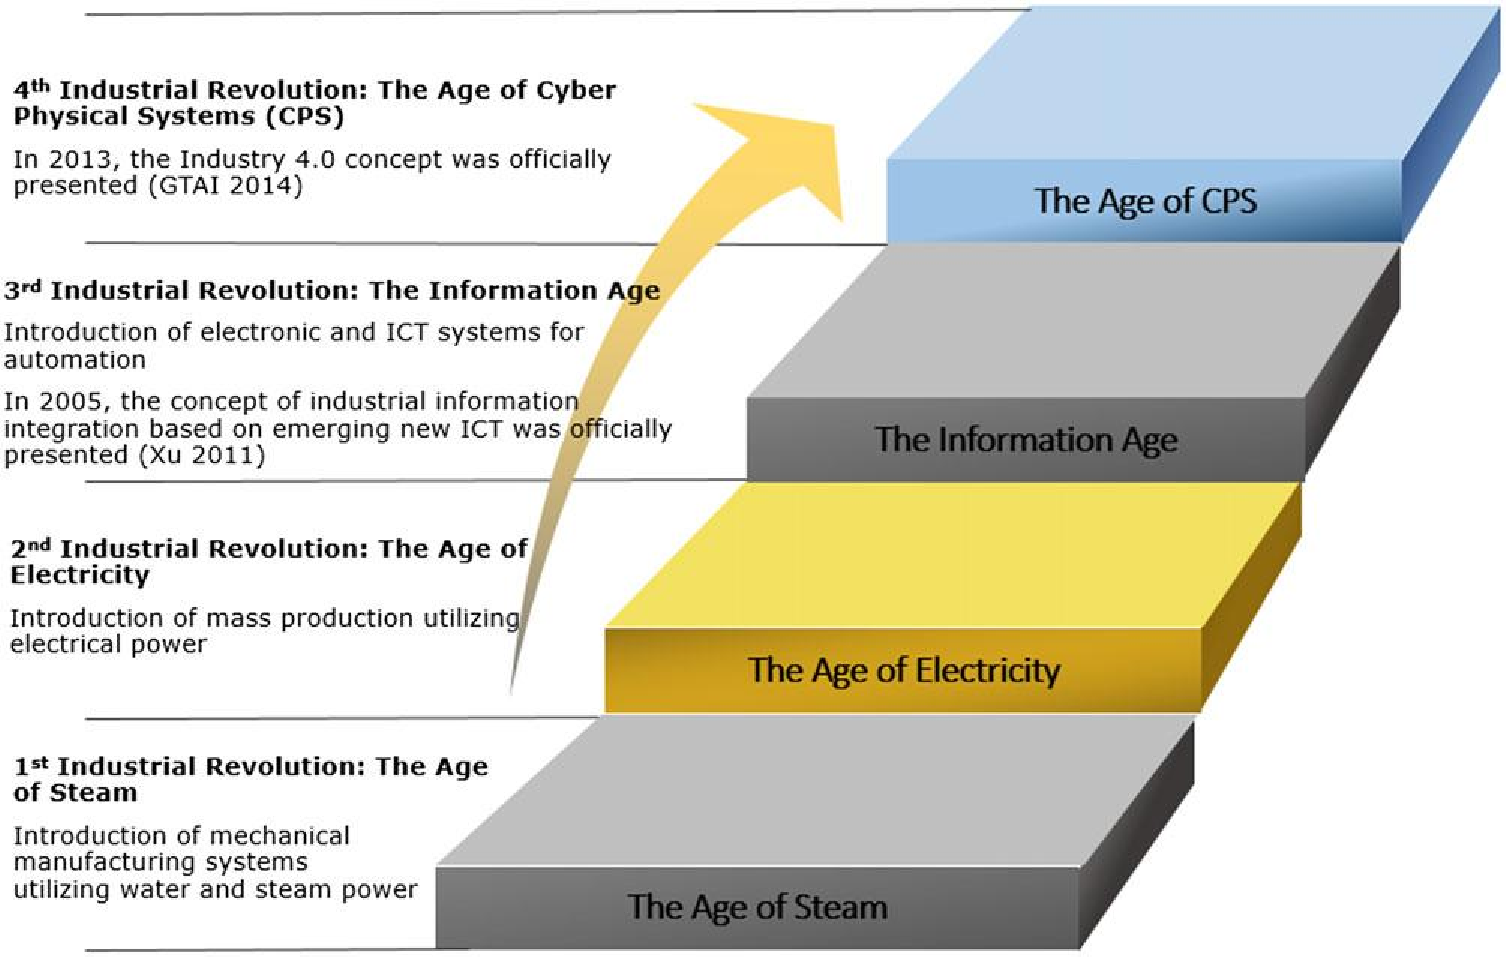
\includegraphics[width=0.88\textwidth]{5-Figures/i4.0_history.pdf} 
    \caption{Evolution from Industry 1.0 to Industry 4.0 \cite{Xu2018}.}
    \label{fig:industry_evolution}
\end{figure}

\subsection{Enabling Technologies of Smart Manufacturing}

Several core technologies work together to make \glspl{CPPS} possible:
\begin{itemize}
    \item \textbf{\glspl{CPS} and \glspl{CPPS}:} Connect physical machinery with sensors, microcontrollers, and communication networks \cite{Abdel-Aty2022}, allowing devices to coordinate actions and collect real-time data \cite{AshtariTalkhestani2019}.
    \item \textbf{\gls{IIOT} and Edge Computing:} Provides reliable networking between shop-floor devices and controllers. Processing data near the machines reduces network load and communication delays \cite{Amthiou2023,Jones2020}.
    \item \textbf{Cloud Computing and \gls{MAAS}:} Enables storage and heavy computing tasks in the cloud, helping companies share production resources and run plant-wide optimization algorithms \cite{Xu2018,Amthiou2023}.
    \item \textbf{Semantic Interoperability and Information Modeling:} Uses standardized data models so that different software tools can share mechanical, electrical, and operational machine data without translation errors \cite{Drath2008,Lu2025}.
    \item \textbf{The \gls{DT}:} Serves as a digital representation of a physical asset, combining real-time sensor data, 3D visualization, and simulation models \cite{Tao2019,Jones2020}.
\end{itemize}

\subsection{Reference Architectural Model Industrie 4.0 (\texorpdfstring{\gls{RAMI}}{RAMI 4.0})}
\label{sec:rami}

Because Industry 4.0 involves many different standards and vendors, Plattform Industrie 4.0 defined \gls{RAMI} (\gls{DIN} \gls{EN} \gls{IEC}~63088). \gls{RAMI} provides a common three-dimensional model to organize industrial assets across their entire lifecycle, factory hierarchy, and software layers \cite{Pajpach2025}, as shown in \Cref{fig:rami40_structure}.

\begin{figure}[htbp]
    \centering
    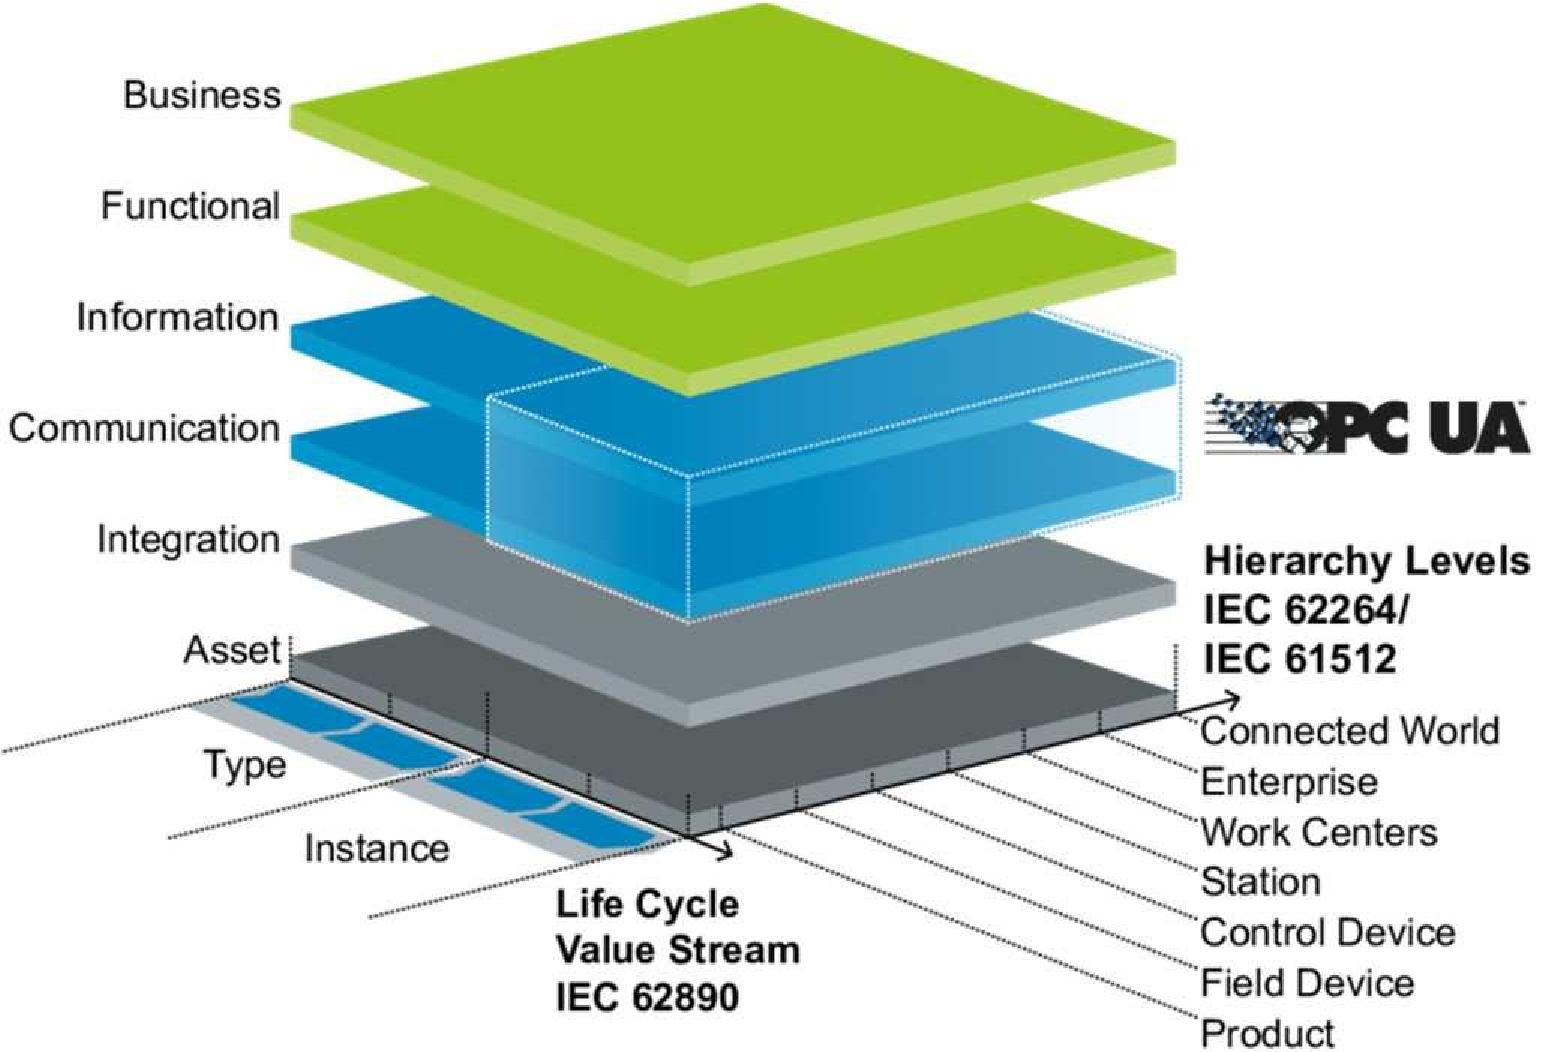
\includegraphics[width=0.88\textwidth]{5-Figures/rami.pdf}
    \caption{The three-dimensional architecture of \gls{RAMI} \cite{Pajpach2025}.}
    \label{fig:rami40_structure}
\end{figure}

The three axes of \gls{RAMI} are defined as follows:
\begin{enumerate}
    \item \textbf{Layers (Vertical Axis):} Divides industrial systems into six viewpoints:
    \begin{itemize}
        \item \textit{Asset Layer:} The physical equipment, including machines, tools, cables, and operators.
        \item \textit{Integration Layer:} The boundary that connects physical hardware to computers using sensors, barcodes, and interfaces.
        \item \textit{Communication Layer:} Communication protocols and network connections, such as \gls{OPCUA}, \gls{MQTT}, and \gls{REST}.
        \item \textit{Information Layer:} Data models, parameters, and variable definitions.
        \item \textit{Functional Layer:} Control logic, application code, and simulation models.
        \item \textit{Business Layer:} Enterprise systems, production orders, and overall process rules.
    \end{itemize}
    
    \item \textbf{Life Cycle and Value Stream (Horizontal Axis):} Based on \gls{IEC}~62890, this axis separates the design phase (``Type'') from the operational phase (``Instance''), helping track an asset from initial engineering to decommissioning.
    
    \item \textbf{Hierarchy Levels (Third Axis):} Extends the standard automation levels (\gls{IEC}~62264 and \gls{IEC}~61512) to include: \textit{Product}, \textit{Field Device}, \textit{Control Device}, \textit{Station}, \textit{Work Centers}, \textit{Enterprise}, and \textit{Connected World}.
\end{enumerate}

In \gls{RAMI}, any asset that has a digital identity and connects to the network is called an \textit{Industry 4.0 Component}. It consists of the physical asset combined with its digital representation, called the \gls{AAS} \cite{Abdel-Aty2022,Pajpach2025}. The \gls{AAS} links the Asset and Integration layers, providing a standard way to access machine data and functions.

%=============================================================================
\section{The Digital Twin Paradigm in Manufacturing}
\label{sec:dt_paradigm}
%=============================================================================

In modern manufacturing, \glspl{DT} have emerged as a core pillar of \glspl{CPPS}. While \glspl{CPPS} define the operational infrastructure integrating sensors, actuators, and distributed control on the shop floor, the \gls{DT} provides the high-fidelity virtual representation and computational intelligence that mirrors, evaluates, and optimizes physical operations \cite{Tao2019,Semeraro2021}. However, despite their clear advantages for monitoring, testing, and optimization, the term is frequently applied loosely across literature to describe any 3D animation or simple dashboard \cite{Kritzinger2018}. A clear taxonomy and historical foundation are therefore essential to distinguish simple virtual representations from fully synchronized \glspl{DT}.

\subsection{Historical Evolution of the Paradigm}
\label{subsec:dt_history}

The idea of using \glspl{DM} to mirror real systems dates back to NASA's Apollo program, where ground simulators replicated spacecraft conditions during missions \cite{Khan2025}. The term ``Digital Twin'' was introduced in 2002 by Michael Grieves for \gls{PLM} \cite{Grieves2014,Jones2020}.

In 2012, NASA and the U.S. Air Force defined the \gls{DT} as an integrated multi-physics simulation of a vehicle or system that uses sensor data and operational history to mirror the life of its physical twin \cite{Shafto2012}. As illustrated in the timeline from \textcite{Khan2025} (\Cref{fig:dt_timeline}), this evolution progressed through key developmental milestones:
\begin{itemize}
    \item \textbf{Conceptual Origins and Theorization (1970 to 2010):} Early ideas emerged from aerospace mirroring in the 1970s, followed by the formal introduction and theorization of the ``Digital Twin'' concept by Michael Grieves in 2002 and 2003 for product lifecycle management.
    \item \textbf{Formal Definition and Consolidation (2010 to 2016):} NASA established the first formal engineering definition in 2012, initiating a period of consolidation where the paradigm expanded into broader manufacturing and cyber-physical automation.
    \item \textbf{Industrial Scaling, Open Standards, and Smart Applications (2021 to Present):} Recent years mark the transition toward large-scale industrial deployment, driven by interoperable open standards, such as \gls{AAS} and \gls{OPCUA}, sustainability objectives, and domain-wide adoption ranging from reconfigurable factories to smart cities \cite{Khan2025,Gil2024}.
\end{itemize}

\begin{figure}[htbp]
    \centering
    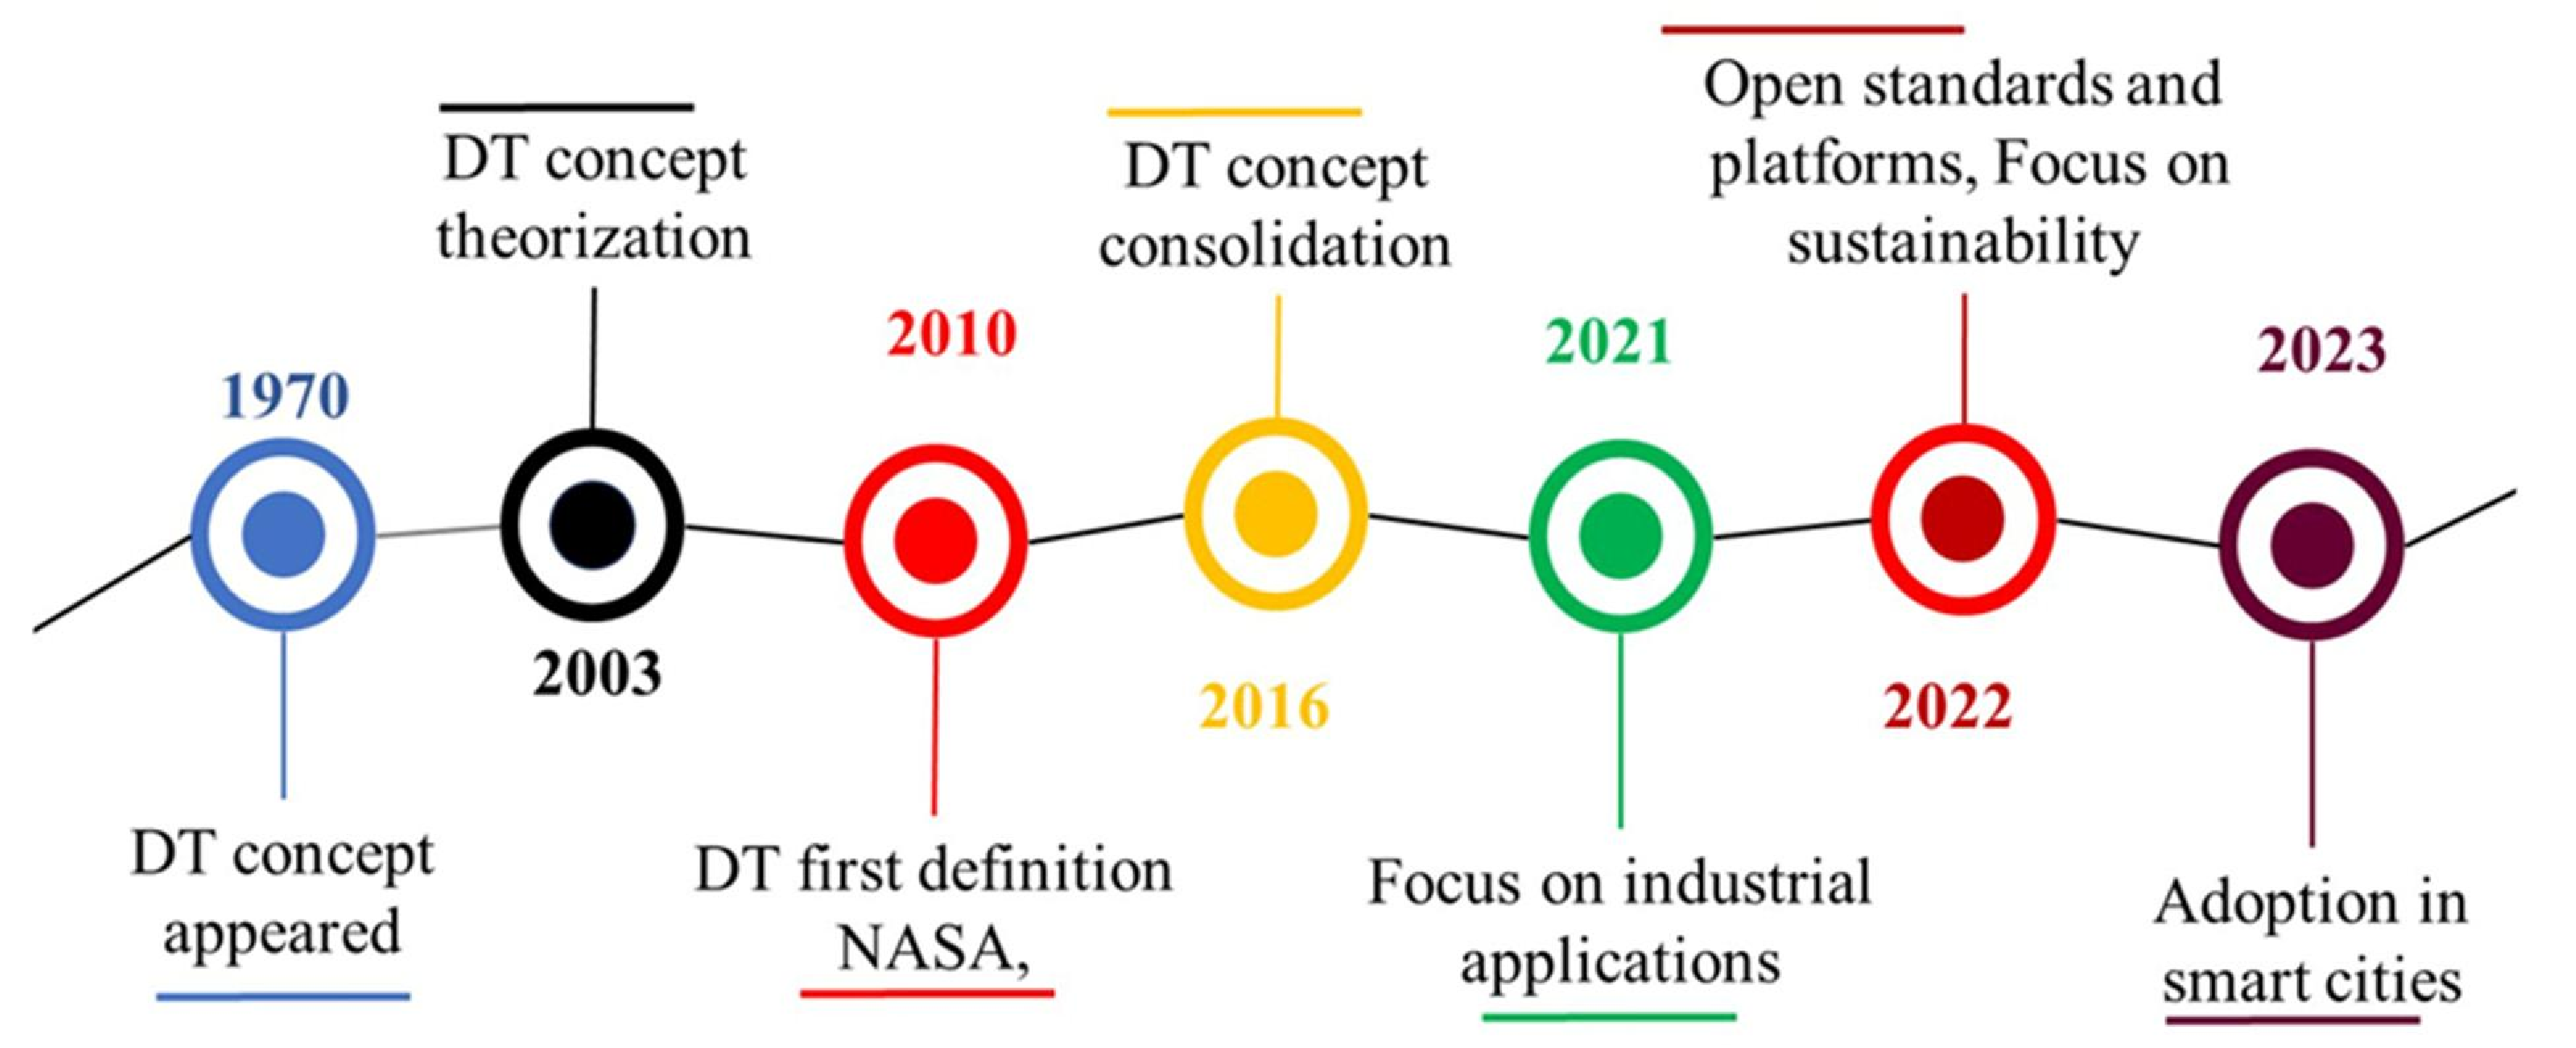
\includegraphics[width=0.88\textwidth]{5-Figures/dt_timeline.pdf}
    \caption{Timeline of \gls{DT} evolution across industrial eras \cite{Khan2025}.}
    \label{fig:dt_timeline}
\end{figure}

\subsection{Taxonomy of Virtual Representations: \texorpdfstring{\gls{DM}}{DM}, \texorpdfstring{\gls{DS}}{DS}, and \texorpdfstring{\gls{DT}}{DT}}
\label{subsec:dt_definition}

To clarify what constitutes a \gls{DT}, this dissertation follows the classification from \textcite{Kritzinger2018}, which separates virtual representations by the level of automated data flow between the physical and digital systems.

\subsubsection{Digital Model (\texorpdfstring{\gls{DM}}{DM})}

A \gls{DM} has manual data exchange in both directions (\Cref{fig:taxonomy_dm}). Static \gls{CAD} drawings, offline kinematic studies, and spreadsheets are typical examples. If changes are made to the physical machine, an engineer must manually update the software model. Likewise, changes made in the model must be implemented by hand on the shop floor.

\subsubsection{Digital Shadow (\texorpdfstring{\gls{DS}}{DS})}

A \gls{DS} has automated, one-way data flow from the physical asset to the digital object. (\Cref{fig:taxonomy_ds}). Sensors and controller tags send live data to the virtual model, so the digital representation updates automatically when the machine moves or changes state. However, the data flow is one-way: the \gls{DS} does not send control commands back to the machine.

\subsubsection{Digital Twin (\texorpdfstring{\gls{DT}}{DT})}

A \gls{DT} has automated, two-way data flow between the physical asset and the digital representation (\Cref{fig:taxonomy_dt}). Sensor readings and controller states update the virtual model automatically, while simulations or decisions made in the digital environment can send commands back to the physical controller to change its operation.

\begin{figure}[htbp]
    \centering
    \begin{subfigure}[b]{0.32\textwidth}
        \centering
        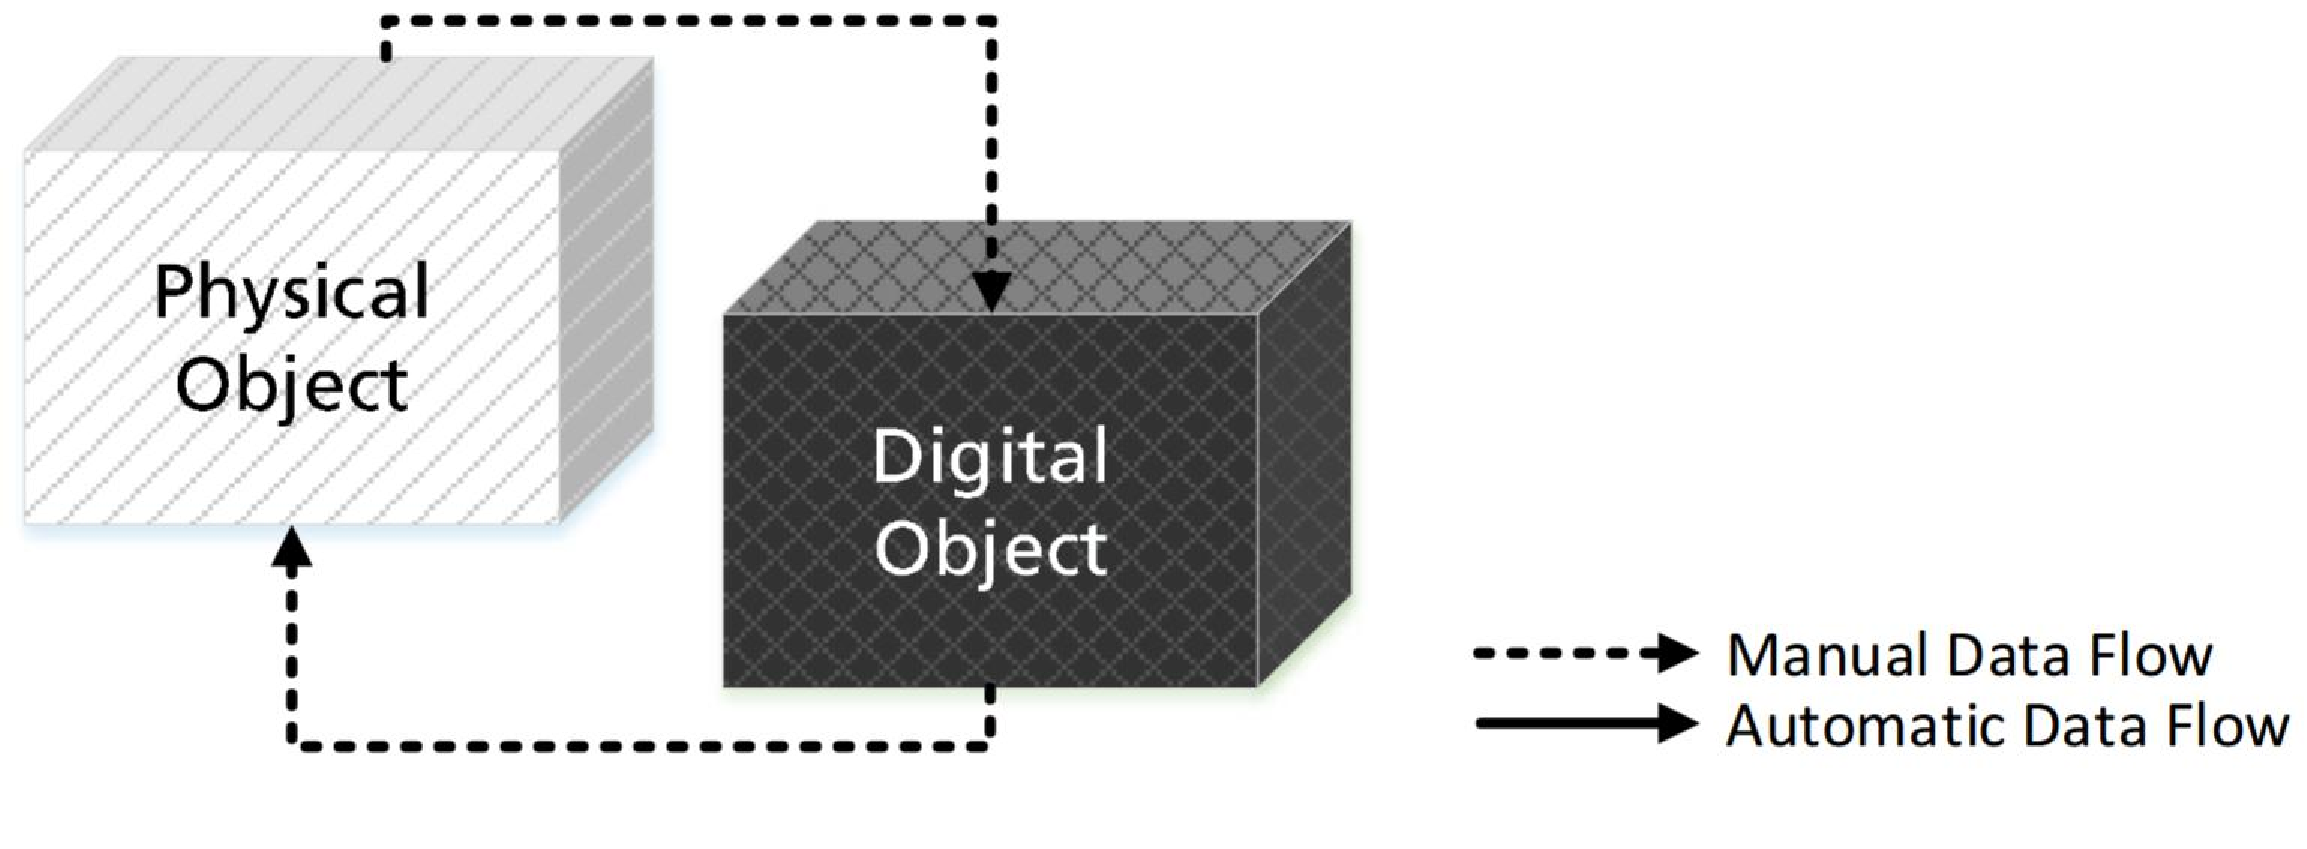
\includegraphics[width=\textwidth]{5-Figures/digital_model_flow.pdf}
        \caption{Digital Model (\gls{DM}).}
        \label{fig:taxonomy_dm}
    \end{subfigure}
    \hfill
    \begin{subfigure}[b]{0.32\textwidth}
        \centering
        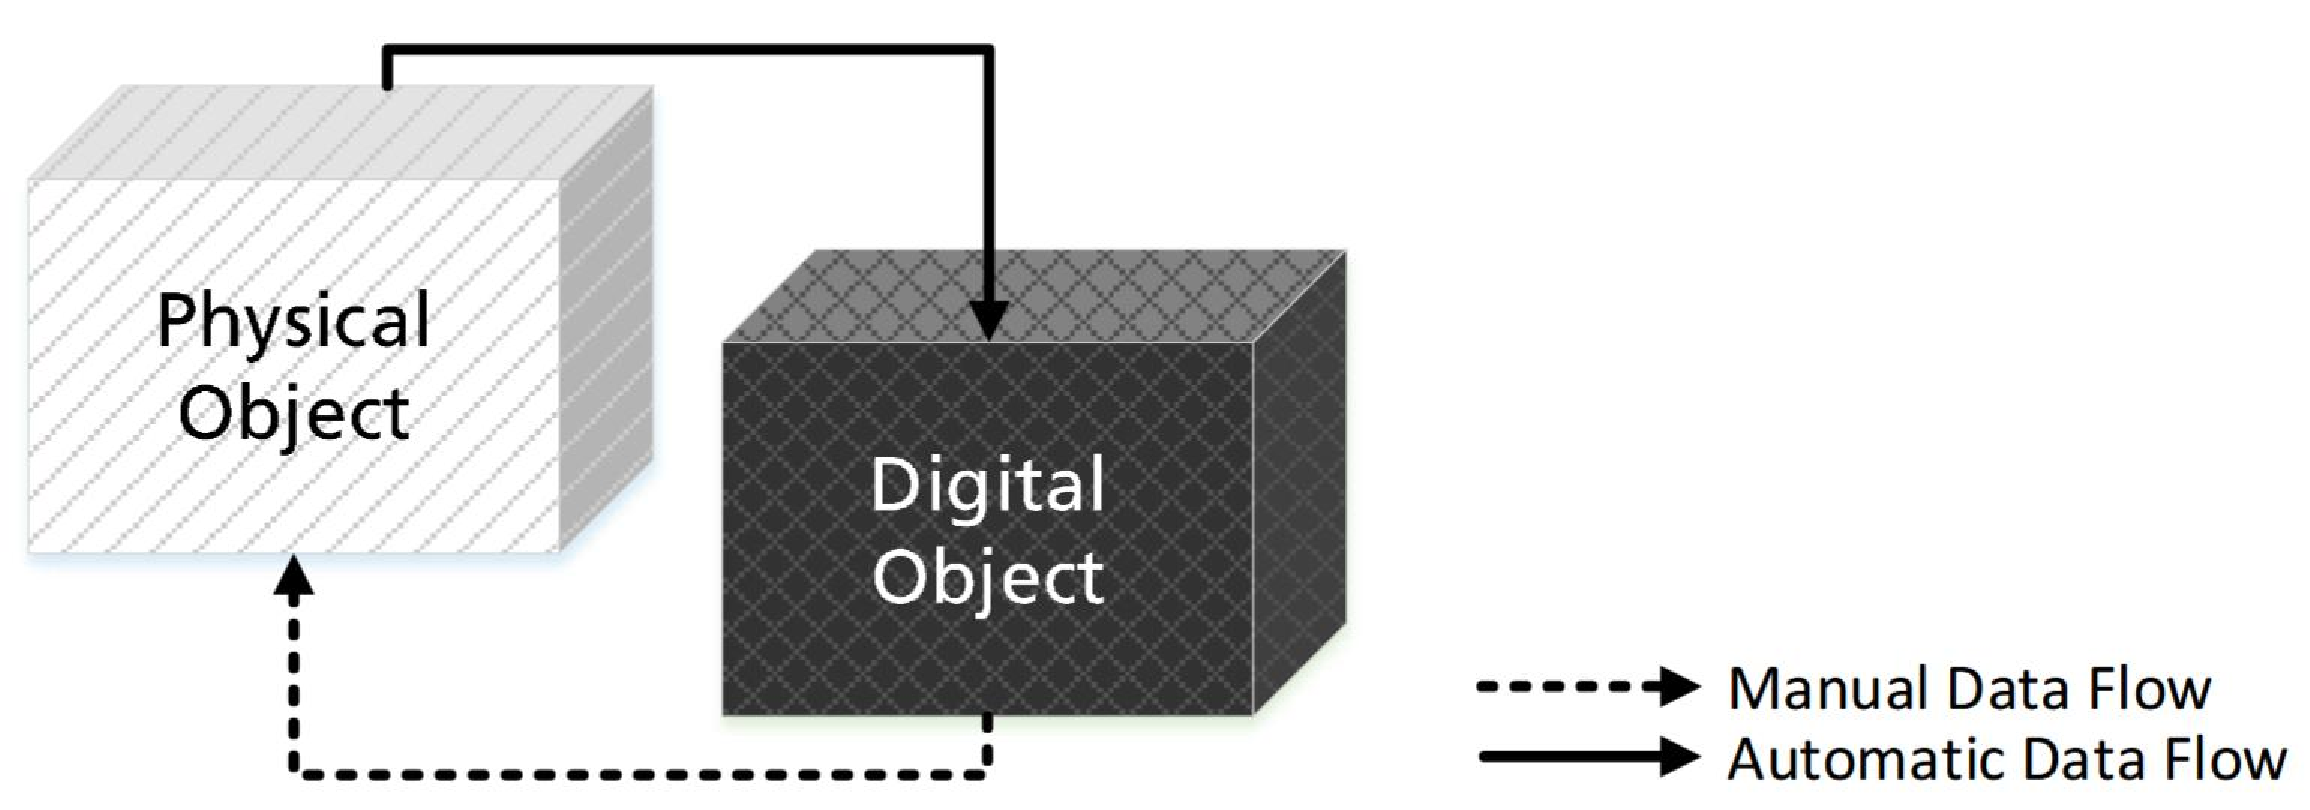
\includegraphics[width=\textwidth]{5-Figures/digital_shadow_flow.pdf}
        \caption{Digital Shadow (\gls{DS}).}
        \label{fig:taxonomy_ds}
    \end{subfigure}
    \hfill
    \begin{subfigure}[b]{0.32\textwidth}
        \centering
        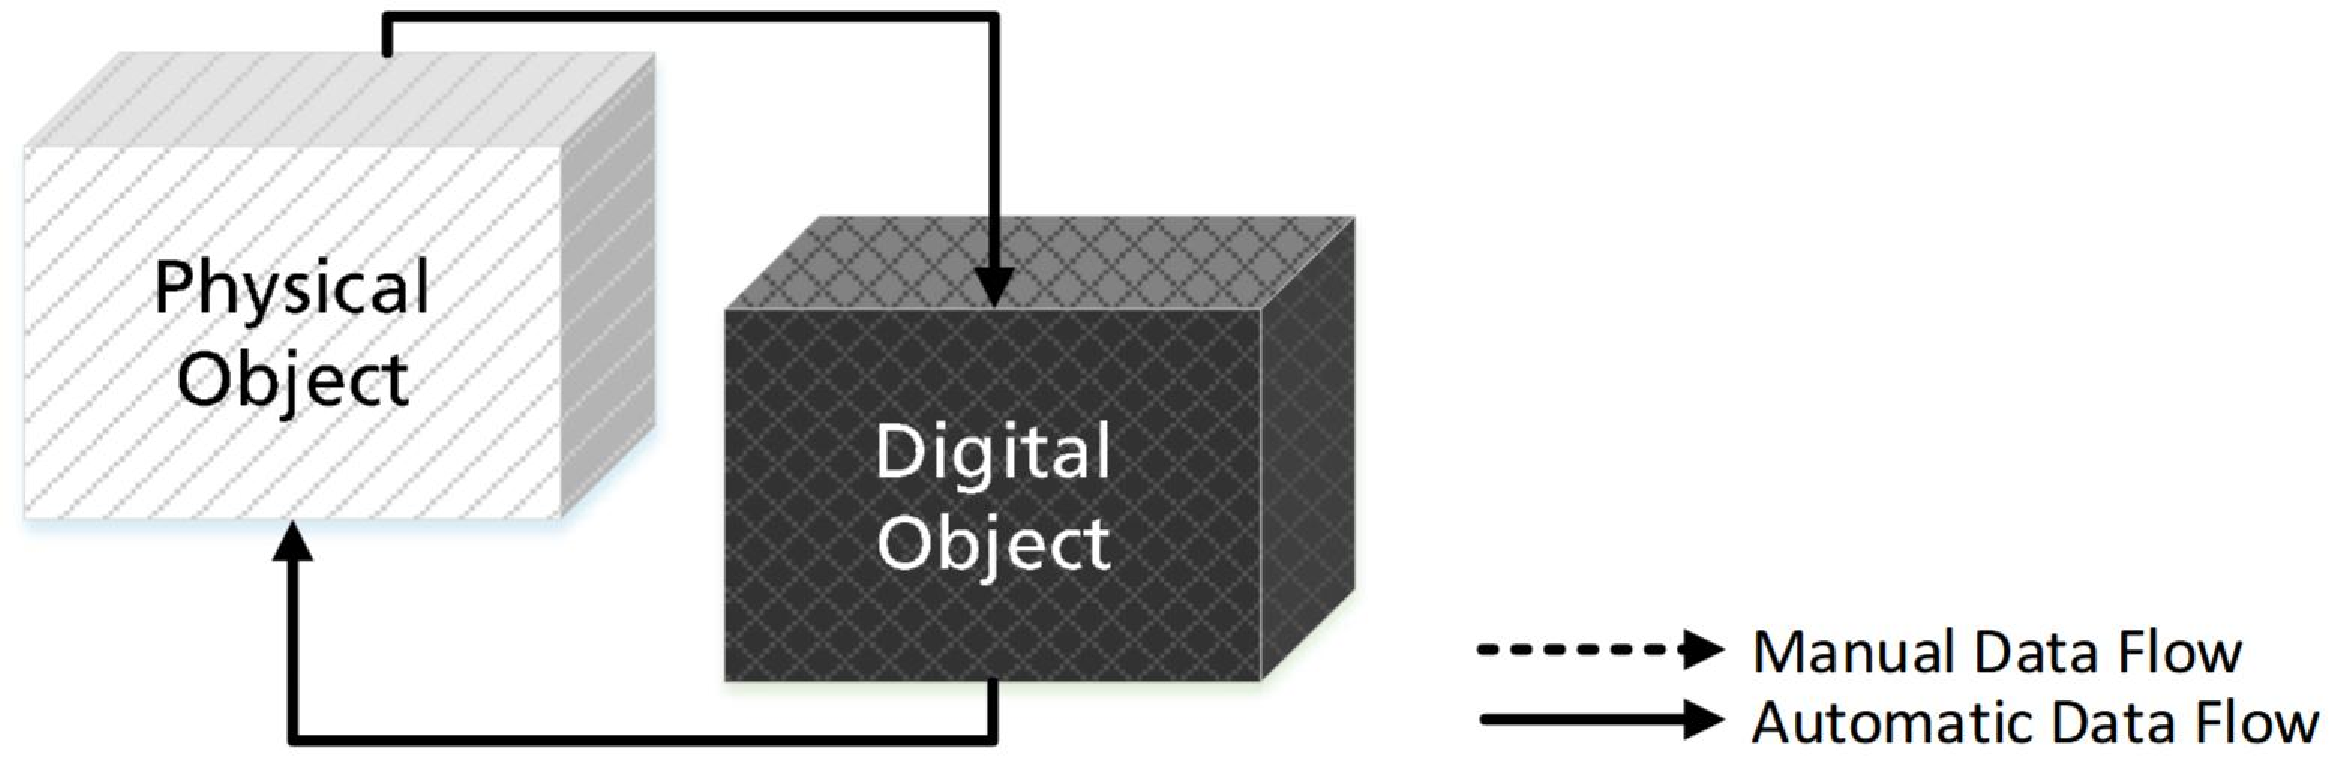
\includegraphics[width=\textwidth]{5-Figures/digital_twin_flow.pdf}
        \caption{Digital Twin (\gls{DT}).}
        \label{fig:taxonomy_dt}
    \end{subfigure}
    \caption{Taxonomy of virtual representations classified by automated data flow: (a) Digital Model, (b) Digital Shadow, and (c) Digital Twin \cite{Kritzinger2018}.}
    \label{fig:dt_taxonomy_comparison}
\end{figure}

Under this definition, many industrial systems marketed as \glspl{DT} are strictly \glspl{DS}, because they only display live telemetry without providing bidirectional control or automated feedback to the physical equipment. Establishing a true \gls{DT} requires closing this loop, enabling both offline virtual testing and real-time bidirectional synchronization.

\subsection{The \texorpdfstring{\gls{DT}}{Digital Twin} Lifecycle}

A \gls{DT} evolves with the machine over its lifecycle \cite{Jones2020,Khan2025}, passing through five main phases:
\begin{enumerate}
    \item \textbf{Design and Modeling:} Starts as a \gls{DM} during early engineering, where \gls{CAD} shapes and expected kinematics are tested before building the machine.
    \item \textbf{Virtual Commissioning:} Tests controller programs against the virtual model before physical installation, using software emulation or physical \glspl{PLC} to catch logic errors early \cite{Striffler2023}.
    \item \textbf{Operational Connectivity:} The machine is installed and connected to the \gls{DT}, establishing live data links to mirror actual movements and states.
    \item \textbf{Optimization and Control:} Operating data is used to improve performance, detect faults, and adjust setpoints on the physical machine \cite{Tao2019}.
    \item \textbf{Reconfiguration and Decommissioning:} When lines are reorganized or parts replaced, the \gls{DT} updates its structure to match the new physical setup.
\end{enumerate}

\subsection{Reference Architectures for Industrial \texorpdfstring{\glspl{DT}}{Digital Twins}}

Several reference architectures have been proposed for \glspl{DT} \cite{Semeraro2021}. \textcite{Tao2019} describe a five-part model: physical entity, virtual entity, services, data, and connection links. \textcite{AshtariTalkhestani2019} present an intelligent architecture that adds software agents for plug-and-produce operations.

In line with these concepts, this dissertation organizes the digital twin workflow into four distinct functional stages:
\begin{itemize}
    \item \textbf{Physical Layer:} Machinery, sensors, conveyors, and controllers operating on the factory shop floor.
    \item \textbf{Authoring Layer:} Tools that ingest raw geometric models and enrich them with kinematic limits, sensor triggers, and operational specifications.
    \item \textbf{Storage and Registry Layer:} Central services that store standardized asset descriptors, maintain device metadata, and provide on-demand endpoint discovery over standard network interfaces.
    \item \textbf{Simulation and Runtime Layer:} The virtual physics and rendering environment that dynamically instantiates assets, executes internal behavior logic, and maintains live two-way synchronization with physical controllers.
\end{itemize}

%=============================================================================
\section{Semantic Modeling and Interoperability Standards}
\label{sec:semantic_interoperability}
%=============================================================================

Building \glspl{DT} automatically requires standard, machine-readable formats. Without standard descriptions for geometry, kinematics, electrical pins, and logic rules, each tool requires custom translation scripts \cite{Ahvanouee2025,Barnard2024}.

Earlier efforts often used \gls{AML} (\gls{IEC}~62714) to share plant structure and 3D files during the engineering phase \cite{Drath2008}. However, \gls{AML} was designed as an offline file format for project handover. It does not provide network \glspl{API} or standard servers for live shop-floor communication \cite{Barnard2024,Ahvanouee2025}.

To provide a standard digital wrapper that works during both design and runtime, Plattform Industrie 4.0 created the \gls{AAS} (\gls{IEC}~63278) \cite{Pajpach2025,Abdel-Aty2022}.

\subsection{\texorpdfstring{\gls{AAS}}{AAS} Architecture and Metamodel}
\label{subsec:aas_deep_dive}

The \gls{AAS} serves as the digital representation of an industrial asset, containing its identification, technical data, and software interfaces \cite{Abdel-Aty2022,Pajpach2025}, as shown in \Cref{fig:aas_introduction}.

\begin{figure}[htbp]
    \centering
    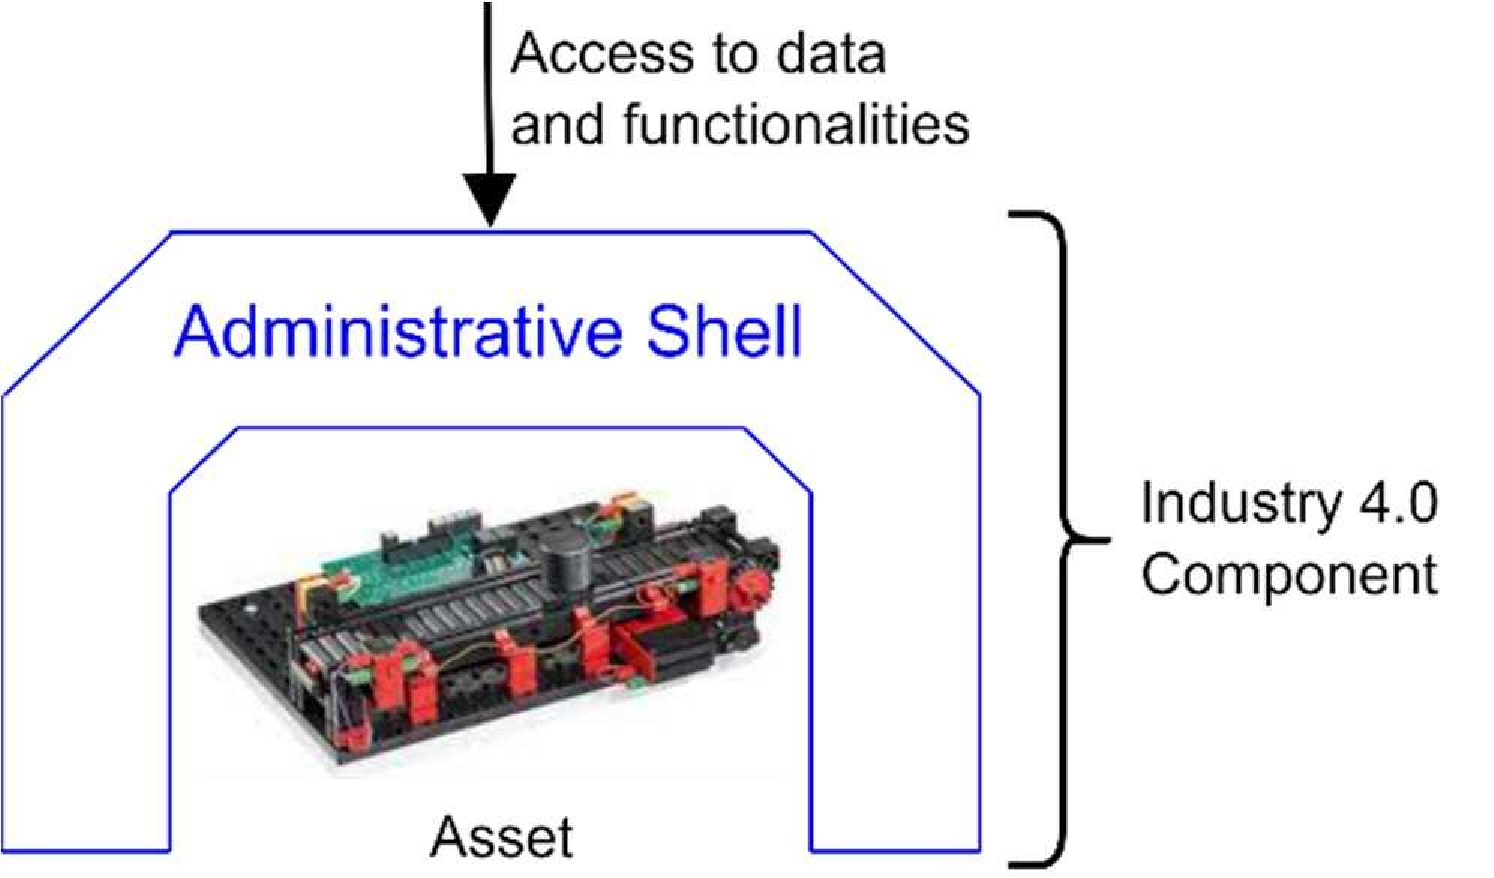
\includegraphics[width=0.85\textwidth]{5-Figures/AAS_introduction.pdf} 
    \caption{Industry 4.0 Component and \gls{AAS} structure \cite{Pajpach2025}.}
    \label{fig:aas_introduction}
\end{figure}

The \gls{AAS} metamodel, standardized under \gls{IEC}~63278 and specified by the \gls{IDTA}, defines a structured hierarchy for representing asset properties \cite{Pajpach2025,Reichardt2024}. It includes the following key parts:
\begin{itemize}
    \item \textbf{\gls{AAS} Container:} The top-level container, identified by a unique ID (\gls{URI} or \gls{UUID}).
    \item \textbf{Asset Information:} States whether the asset is a generic product type or a specific physical unit on the shop floor.
    \item \textbf{Submodel:} A group of related properties for a specific domain, such as identification, technical specs, or kinematics. Each submodel has an identifier and a reference to a standardized semantic definition (such as \gls{ECLASS} or \gls{IDTA} templates).
    \item \textbf{Submodel Elements:} The actual data fields within a submodel \cite{Reichardt2024,Barnard2024}:
    \begin{itemize}
        \item \textit{Property}: Stores a single value, such as a number, text, or boolean.
        \item \textit{MultiLanguageProperty}: Stores text in multiple languages.
        \item \textit{Range}: Sets minimum and maximum limits for a numerical value.
        \item \textit{File} and \textit{Blob}: References or embeds files, such as 3D meshes, user manuals, or drawings.
        \item \textit{SubmodelElementCollection} and \textit{SubmodelElementList}: Groups multiple submodel elements together.
        \item \textit{Operation}: Defines invokable functions with input and output parameters.
    \end{itemize}
\end{itemize}

\subsection{Standardized Submodel Templates and \texorpdfstring{\gls{IDTA}}{IDTA} Specifications}

The main benefit of the \gls{AAS} is that different systems can read and interpret data without custom integration code when adhering to standardized \textit{Submodel Templates} released by the \gls{IDTA} \cite{Abdel-Aty2022,Ahvanouee2025}. Well-established templates frequently analyzed in literature include:
\begin{itemize}
    \item \textbf{Digital Nameplate (\gls{IEC}~61406):} Replaces physical nameplates with machine-readable serial numbers, manufacturer details, and conformity marks.
    \item \textbf{Technical Data:} Provides a standardized frame for operating limits, dimensions, voltages, and ratings for industrial equipment.
    \item \textbf{Contact Information:} Standardizes manufacturer and service contact details for maintenance and lifecycle support.
\end{itemize}

While these templates cover general information, templates for real-time physics, kinematics, and control logic are still emerging in the literature \cite{Pajpach2025,Perez2025}. This is one of the main areas where this dissertation defines and tests custom submodel structures.

\subsection{Portable Packaging: The \texorpdfstring{\gls{AASX}}{AASX} Container}

To make it easy to share \gls{DT} assets across different computers and tools, the standard defines the \gls{AASX} package (\gls{IEC}~63278-1). The \gls{AASX} format uses the \gls{OPC}, the same container format used by common office documents.

An \gls{AASX} package bundles:
\begin{enumerate}
    \item The \gls{AAS} and its submodels saved as \gls{JSON} or \gls{XML}.
    \item Embedded binary files, such as 3D meshes (\gls{GLB}/\gls{glTF}), wiring diagrams, and icons.
    \item Relationship files that link the data together.
\end{enumerate}

Using \gls{AASX} allows an asset to be distributed as a single file. An application can download the package and immediately load its 3D model, joints, pin mappings, and connection addresses without needing extra files.

\Cref{fig:pajpach_aasx_conveyor} illustrates how a physical conveyor module is traditionally modeled inside the standard \gls{IDTA} toolchain using the official \gls{AASX} Package Explorer \cite{Pajpach2025}. In conventional workflows, the automation engineer must manually populate extensive hierarchical tables, defining properties, ranges, and submodel element collections without visual feedback or spatial awareness of the physical asset.

\begin{figure}[htbp]
    \centering
    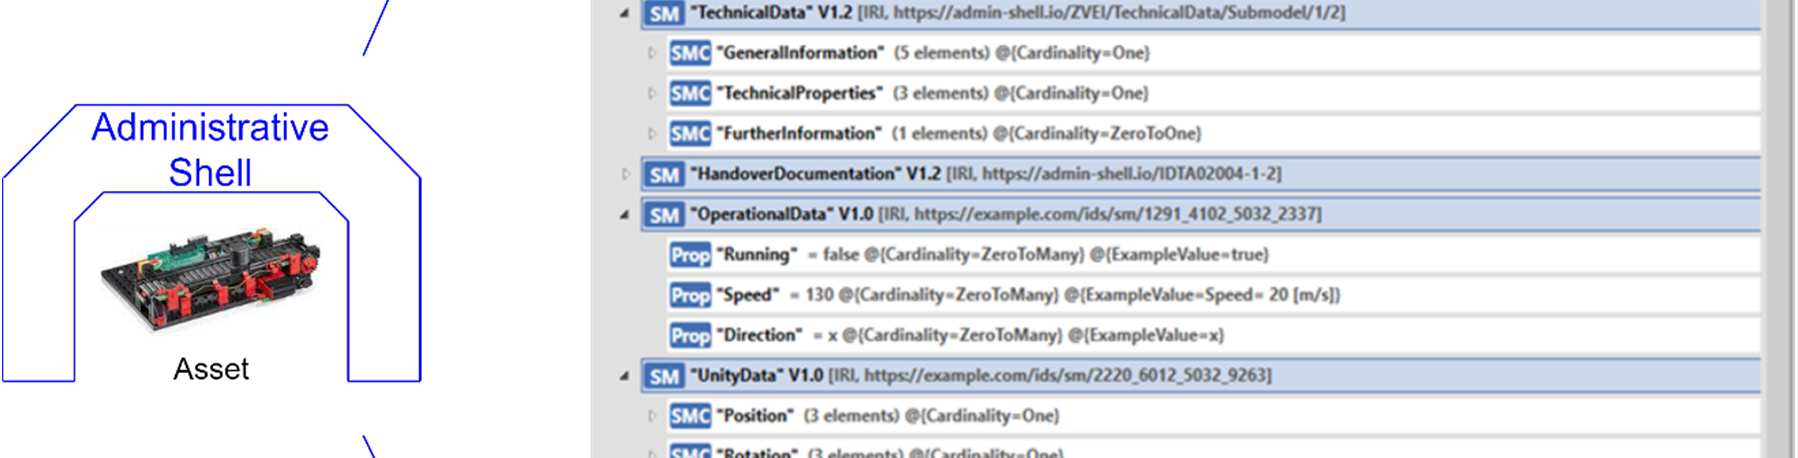
\includegraphics[width=0.92\textwidth]{5-Figures/pajpach_aasx_conveyor}
    \caption{Digital description of a modular conveyor within the official \gls{AASX} Package Explorer \cite{Pajpach2025}.}
    \label{fig:pajpach_aasx_conveyor}
\end{figure}

\subsection{\texorpdfstring{\gls{AAS}}{AAS} Middleware and Toolchains}

To use \glspl{AAS} during operation, server software must host them and provide network access through \gls{REST}, \gls{HTTP}, and \gls{MQTT}:
\begin{itemize}
    \item \textbf{Eclipse BaSyx:} An open-source implementation of Plattform Industrie 4.0. It provides modular services including:
    \begin{itemize}
        \item \textit{AAS Server:} Hosts \gls{AAS} data and provides standard \gls{REST} endpoints.
        \item \textit{AAS Registry:} Keeps track of where each asset is hosted so applications can find them.
        \item \textit{DataBridge:} Connects \gls{AAS} properties directly to field protocols like \gls{OPCUA} and \gls{MQTT} \cite{Perez2025,Caldana2025}.
    \end{itemize}
    \item \textbf{AASX Package Explorer:} A graphical tool used to create, inspect, and validate \gls{AASX} files \cite{Pajpach2025}.
    \item \textbf{Development Libraries:} Open-source libraries such as aas-core and basyx-python-sdk allow software applications to read and write \gls{AAS} data across Python, C\#, and TypeScript.
\end{itemize}

%=============================================================================
\section{Virtual Environments and Game Engines in Industry 4.0}
\label{sec:game_engines_vc}
%=============================================================================

While older factory monitoring used flat 2D screens, modern systems increasingly rely on 3D environments that accurately display robot motions, part transfers, and layout configurations \cite{Pajpach2022,Zheng2024}.

\subsection{Game Engines for Industrial Simulation}

Real-time game engines, especially Unity and Unreal Engine, have become popular choices for industrial \glspl{DT}, offering several practical benefits:
\begin{enumerate}
    \item \textbf{Rendering Speed:} Game engines are optimized for graphics hardware, rendering complex 3D scenes smoothly at 60 \gls{FPS} or higher.
    \item \textbf{Flexible Scripting:} Unlike closed industrial simulation software, engines like Unity provide open programming environments (C\#) that make it straightforward to add network libraries for \gls{MQTT}, \gls{OPCUA}, or \gls{REST} \glspl{API}.
    \item \textbf{Lower Licensing Barriers:} Standard game engine licenses are generally more accessible than specialized industrial simulation software (such as Siemens Tecnomatix) \cite{Pajpach2022}.
    \item \textbf{Cross-Platform Support:} Projects can run on desktop computers, web browsers, or \gls{XR} headsets \cite{Garcia2025}.
\end{enumerate}

Platforms like NVIDIA Omniverse (based on the \gls{USD} format) are also growing, but Unity remains widely used in research due to its lightweight runtime, physics engine, and extensive documentation \cite{Alexopoulos2025,Garcia2025,Pajpach2023}.

\subsection{Bridging \texorpdfstring{\gls{CAD}}{CAD} and Real-Time Graphics}

A common problem identified in the literature is that mechanical \gls{CAD} models are not designed for real-time simulation engines \cite{Chowdhury2025,Striffler2023,Zheng2024}.

\gls{CAD} files use mathematical shapes (\glspl{BRep}) to store exact production details, like screw threads and internal components. In contrast, game engines need lightweight triangle meshes to keep high frame rates. Preparing \gls{CAD} models for real-time simulation typically involves three main steps \cite{Chowdhury2025,Striffler2023}:
\begin{itemize}
    \item \textbf{Tessellation and Simplification:} Converting curved surfaces into triangles and reducing polygon counts while keeping the visual shape.
    \item \textbf{Removing Internal Parts:} Deleting hidden parts, like screws and bolts, that are not needed for motion or collisions.
    \item \textbf{Standard Export Formats:} Saving meshes into open formats like \gls{glTF}/\gls{GLB} 2.0, which load quickly and keep the model hierarchy organized.
\end{itemize}

\subsection{Behavioral Simulation and \texorpdfstring{\gls{VC}}{Virtual Commissioning}}

Beyond visual display, a \gls{DT} must replicate machine motion and sensor behavior \cite{Striffler2023}. This is essential for \gls{VC}, where controller programs are tested against a virtual model before the physical machine is assembled \cite{Lee2014}.

Common \gls{VC} setups include:
\begin{itemize}
    \item \textbf{\gls{MIL}:} Controller logic and mechanical dynamics are simulated together within early conceptual design tools.
    \item \textbf{\gls{SIL}:} Both the machine kinematics and the \gls{PLC} runtime code are simulated in software on a computer.
    \item \textbf{\gls{HIL}:} A physical \gls{PLC} is wired or networked to the simulation computer. The game engine feeds virtual sensor signals to the \gls{PLC} inputs and reads the \gls{PLC} actuation outputs.
\end{itemize}

As classified by \textcite{Striffler2023}, \Cref{fig:striffler_vc_configs} outlines the spectrum of virtual commissioning topologies, contrasting purely software-based simulation loops (such as \gls{MIL} and \gls{SIL}) against real-time physical \gls{HIL} coupling, where physical controllers exchange sensor and actuator signals with the virtual model.

\begin{figure}[htbp]
    \centering
    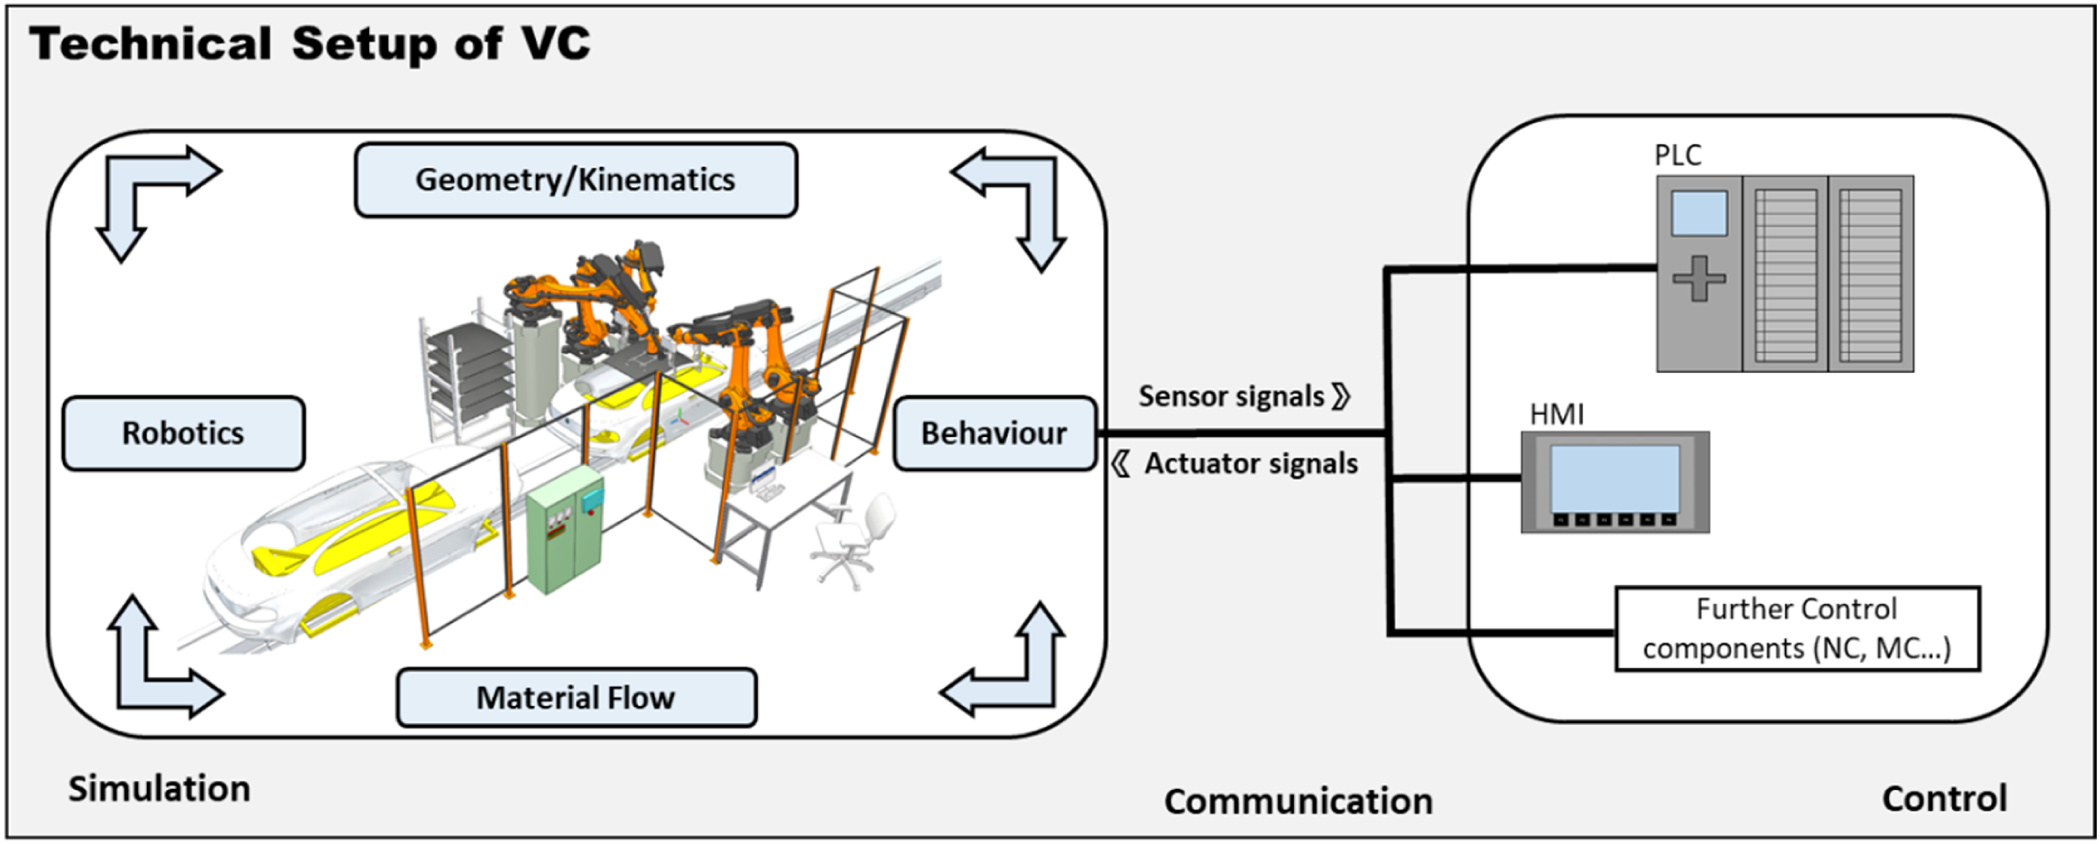
\includegraphics[width=0.92\textwidth]{5-Figures/striffler_vc_technical_configurations.jpeg}
    \caption{Technical configurations of \gls{VC}: \gls{MIL}, \gls{SIL}, and \gls{HIL} \cite{Striffler2023}.}
    \label{fig:striffler_vc_configs}
\end{figure}

When complex multi-body physics equations are needed, game engines can use the \gls{FMI} standard \cite{Chowdhury2025}. External simulation models compiled as \glspl{FMU} compute the physics, while the game engine handles visualization. \textcite{Juhlin2022} showed how combining \glspl{AAS} with \glspl{FMU} allows cloud-based simulation of motor drives.

\subsection{Industrial Communication in the Game Engine Loop}

Connecting a game engine to industrial hardware requires care with thread timing. Game engines run on a continuous loop that updates graphics every frame (often 60 to 120 times per second) and updates physics at fixed intervals (typically 50~Hz, or every 20~ms).

If network queries (\gls{OPCUA}, \gls{MQTT}, or \gls{REST}) run directly on the main graphics thread, network delays or packet retransmissions can block the engine loop and degrade rendering performance \cite{Pajpach2022}.

To ensure smooth runtime performance, industrial game engine architectures decouple communication onto background worker threads \cite{Pajpach2022,Pajpach2023,Garcia2025}:
\begin{enumerate}
    \item \textbf{Background Threads:} Network listeners run on separate threads or coroutines, receiving incoming sensor and controller frames asynchronously.
    \item \textbf{Thread-Safe Data Exchange:} Incoming states are placed into thread-safe queues or buffers to safely transfer data to Unity's main thread.
    \item \textbf{Decoupled Physics Execution:} The engine's fixed physics loop reads the buffered states at regular intervals, preventing communication latency from stalling visual and mechanical simulation.
\end{enumerate}

\Cref{fig:pajpach_unity_dataflow} shows an example architecture from \textcite{Pajpach2023}, where Unity 3D retrieves 3D models from an \gls{AAS} repository and exchanges runtime signals with a physical \gls{PLC} through an \gls{OPCUA} server and Node-RED middleware. Similarly, \textcite{Garcia2025} used Unity 3D with BaSyx \gls{AAS} data spaces for remote line monitoring.

\begin{figure}[htbp]
    \centering
    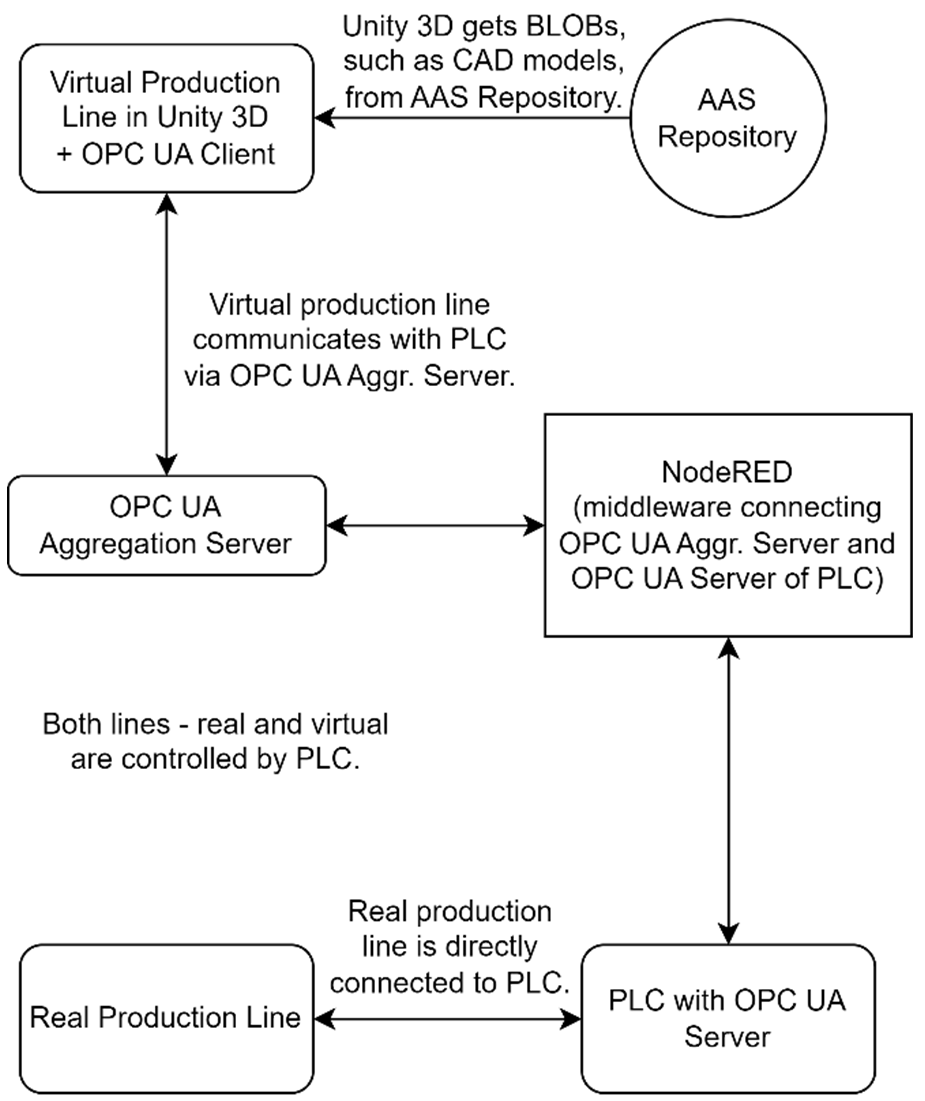
\includegraphics[width=0.72\textwidth]{5-Figures/pajpach_dt_unity_dataflow.png}
    \caption{Architecture and data flow in an educational \gls{DT} using Unity 3D, \gls{AAS}, and \gls{OPCUA} \cite{Pajpach2023}.}
    \label{fig:pajpach_unity_dataflow}
\end{figure}

%=============================================================================
\section{Automated Generation of \texorpdfstring{\glspl{DT}}{Digital Twins}}
\label{sec:automated_dt_generation}
%=============================================================================

While \glspl{DT} offer clear benefits, the engineering effort required to build and maintain them remains high, especially for smaller manufacturers \cite{Alexopoulos2025,Schaper2025}.

\subsection{Bottlenecks in Manual Workflows}

Traditional \gls{DT} development is mostly manual. As shown in \Cref{fig:toolchain_fragmentation}, engineering data is split across different tools \cite{Schaper2025}: mechanical engineers work in \gls{CAD}, electrical engineers design schematics in \gls{ECAD}, software developers write \gls{PLC} code in vendor tools, and asset data is stored in \gls{PLM} or \gls{MES} databases.

\begin{figure}[htbp]
    \centering
    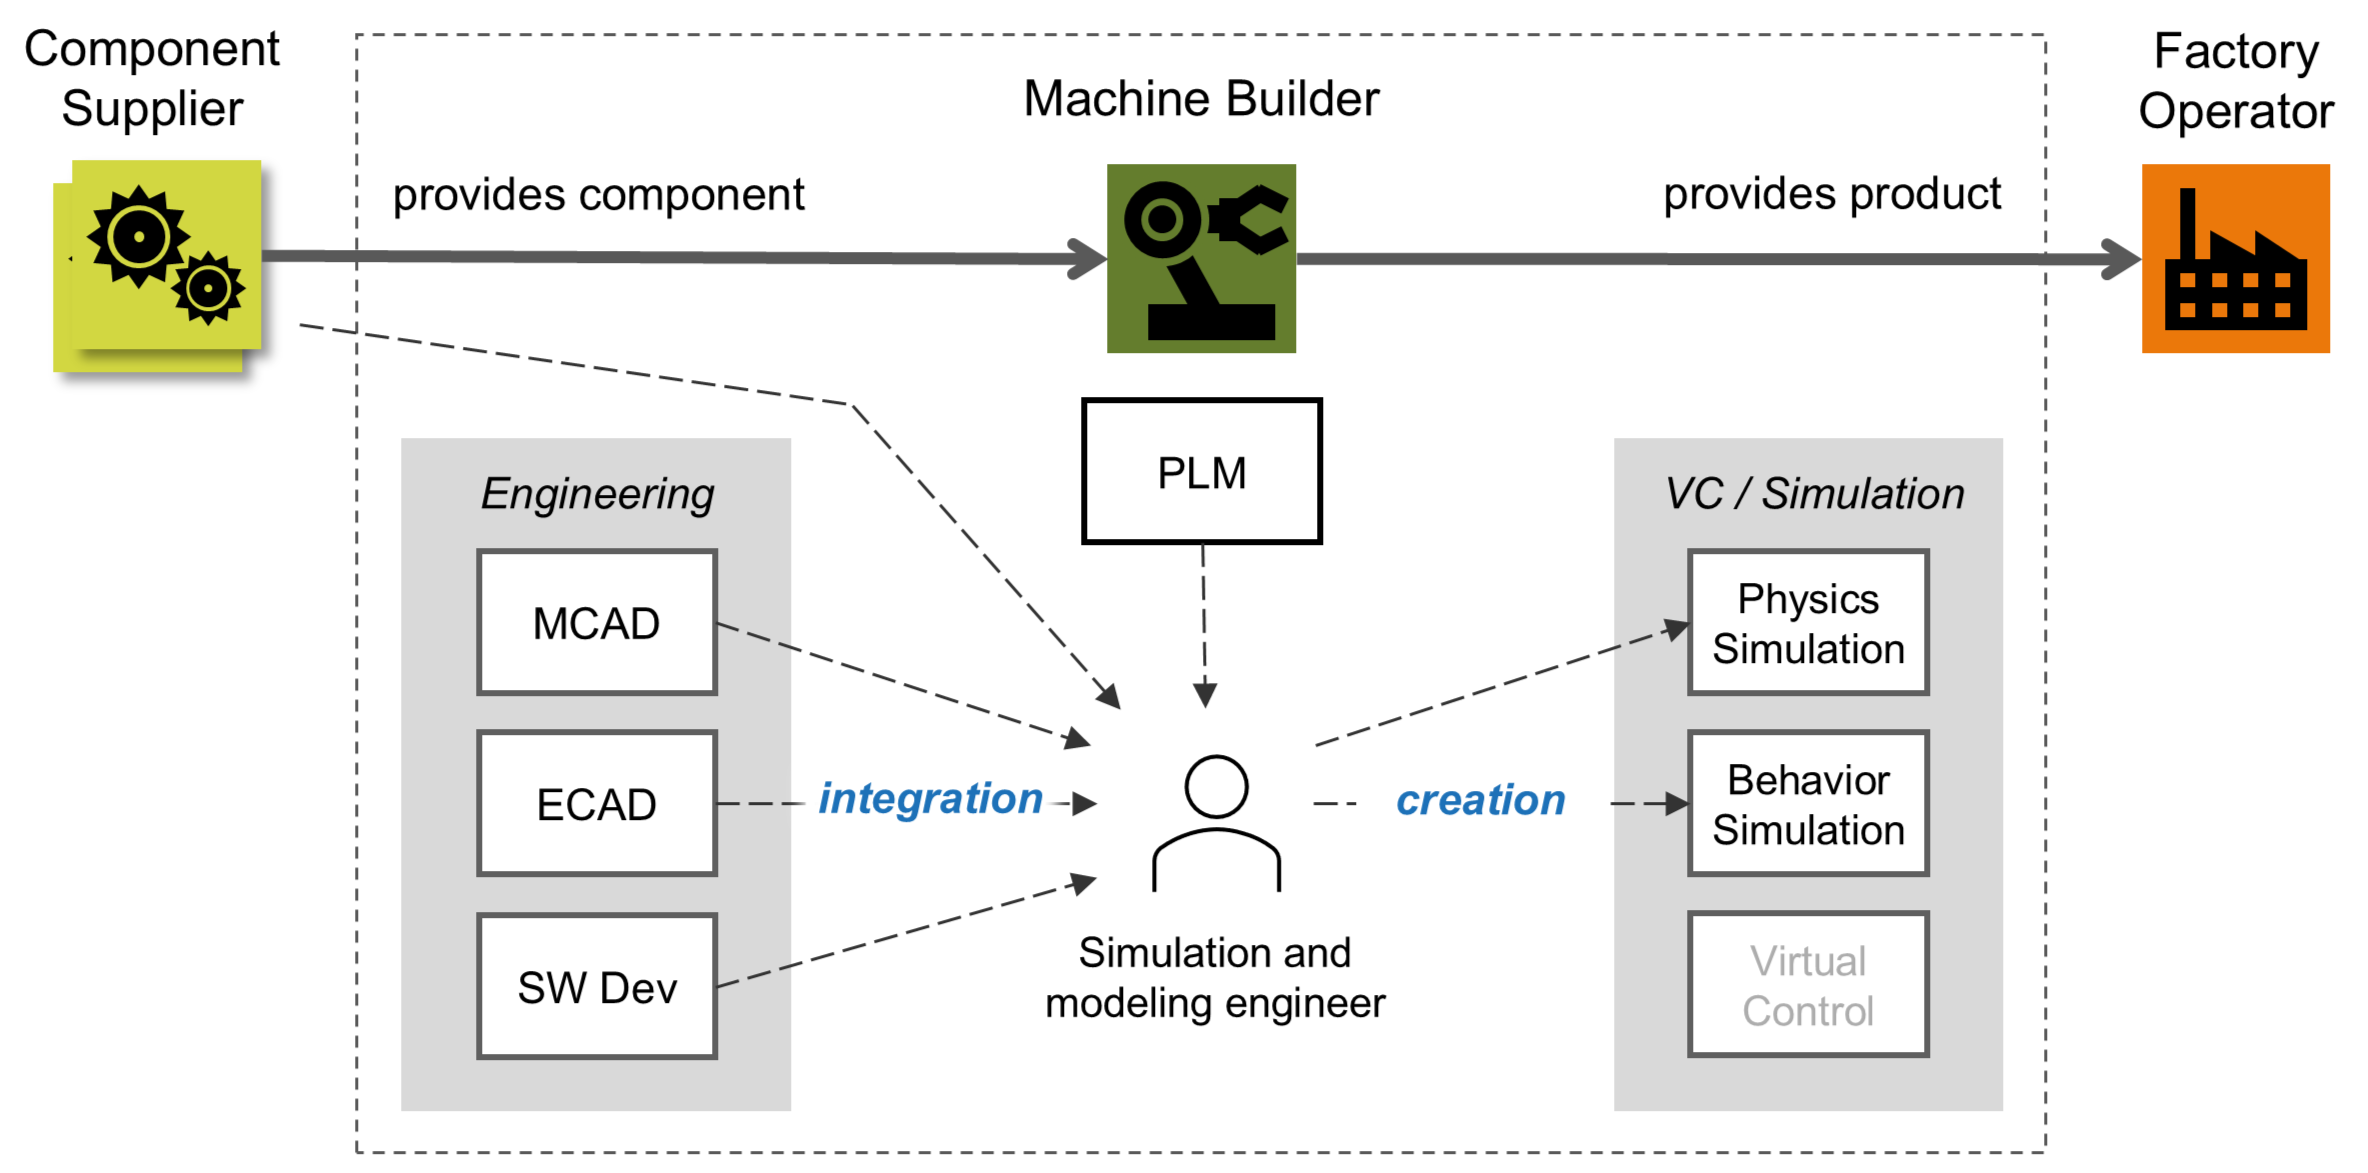
\includegraphics[width=0.88\textwidth]{5-Figures/schaper_toolchain_bottleneck.png}
    \caption{Data fragmentation across engineering tools in machine development \cite{Schaper2025}.}
    \label{fig:toolchain_fragmentation}
\end{figure}

To build a simulation model, an engineer has to collect all these files, import 3D meshes into the engine, set up parent-child relationships, configure joint limits, and manually connect virtual sensors to \gls{PLC} addresses \cite{Alexopoulos2025,Koch2024}.

This manual approach has three main drawbacks:
\begin{enumerate}
    \item \textbf{High Time and Cost:} Building a model for a single workstation can take several weeks of engineering work \cite{Garcia2023}.
    \item \textbf{Risk of Configuration Errors:} Connecting hundreds of signal addresses by hand easily leads to mistakes that can cause simulation bugs.
    \item \textbf{Maintenance Delays:} In reconfigurable factories, machines are frequently moved or swapped. If the simulation model is not updated immediately, it quickly becomes outdated and unreliable \cite{Ahvanouee2025,Herzog2025}.
\end{enumerate}

To address these issues, recent research focuses on automating \gls{DT} creation. Existing methods generally follow model-driven, data-driven, or \gls{AI}-based approaches.

\subsection{Model-Driven Approaches}

Model-driven approaches use existing engineering files as the source to build the \gls{DT} components, 3D scenes, and signal connections automatically \cite{Luder2020,Ahvanouee2025}.

Examples include:
\begin{itemize}
    \item \textbf{AutomationML-Based Methods:} \textcite{Alexopoulos2025} parse \gls{AML} files containing plant topology and device types to instantiate 3D machines and set up communication drivers in Unity, as shown in \Cref{fig:alexopoulos_architecture}. \textcite{Chowdhury2025} extract part relationships and mass properties from \gls{CAD} files to assemble motion models in Unreal Engine using \gls{FMI}.
    \item \textbf{AAS-Based Configuration:} \textcite{Pretz2025} use \gls{AAS} descriptions to configure \glspl{AMR} automatically. \textcite{Ahvanouee2025} use \gls{AAS} submodels to exchange data between different engineering tools across supply chain partners.
    \item \textbf{SysML Models:} \textcite{Heermann2024} use textual \gls{SysML}~v2 models to generate \gls{DT} software modules and \gls{MQTT} topic structures.
    \item \textbf{ECAD and Multi-Physics Synthesis:} \textcite{Schaper2025} parse electrical and fluid schematics together with \gls{AAS} component data to connect \gls{FMU} simulation blocks automatically. \textcite{Koch2024} similarly generate simulation models using structured component descriptions.
    \item \textbf{Automatic AAS Assembly:} \textcite{Gollner2022} present a method that queries equipment databases to generate populated \gls{AAS} files automatically. \textcite{Perez2025} generate Eclipse BaSyx DataBridge configs directly from interface submodels.
\end{itemize}

\begin{figure}[htbp]
    \centering
    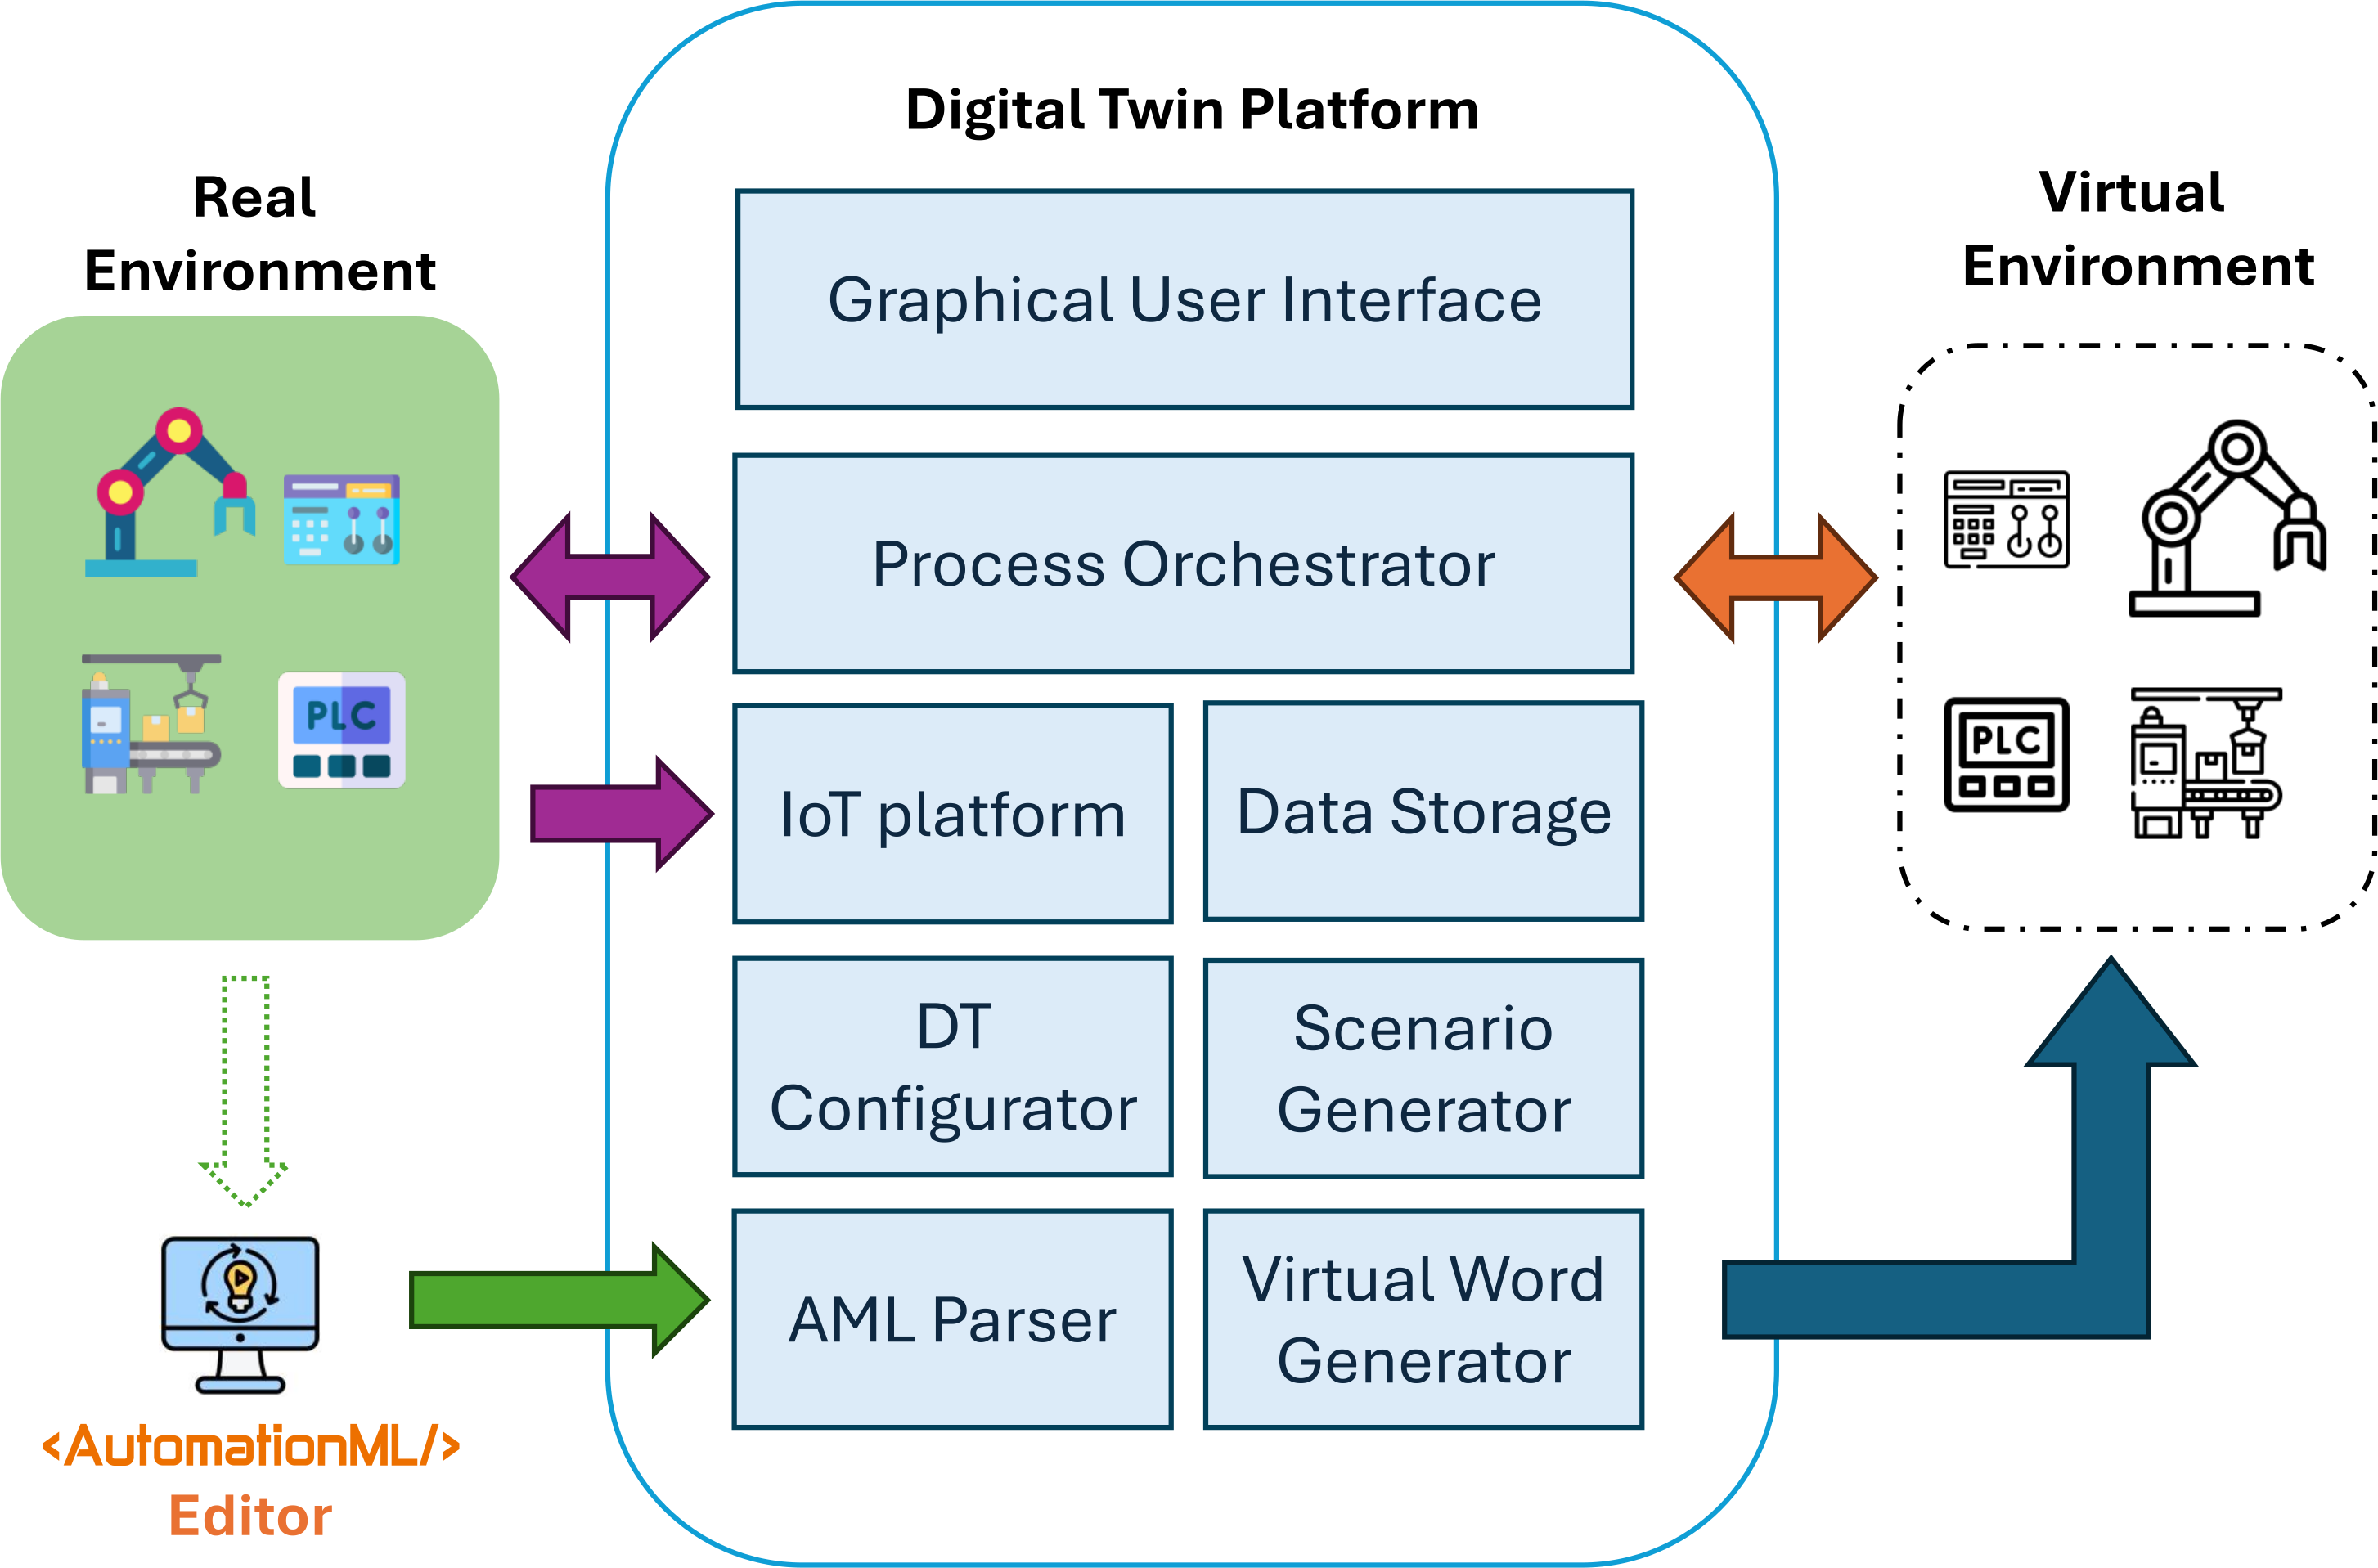
\includegraphics[width=0.88\textwidth]{5-Figures/alexopoulos_dt_architecture.png}
    \caption{Architecture of the model-based platform for automated \gls{DT} generation \cite{Alexopoulos2025}.}
    \label{fig:alexopoulos_architecture}
\end{figure}

Model-driven methods provide reliable, deterministic results because they follow validated engineering designs. However, they require clean, up-to-date source files.

\subsection{Data-Driven Approaches}

In older factories where machines lack up-to-date \gls{CAD} or design files, data-driven methods discover the \gls{DT} structure from historical and live sensor data \cite{Lugaresi2021,Garcia2023}:
\begin{itemize}
    \item \textbf{Process Mining from Event Logs:} \textcite{Lugaresi2021} apply process mining to timestamped machine logs to determine routing, part flows, and buffer queues, building discrete event simulation models without design drawings.
    \item \textbf{Machine Learning Surrogates:} \textcite{Garcia2023} train machine learning models on sensor readings to estimate energy use, creating behavior models directly from measurement data.
\end{itemize}

Data-driven methods work well when engineering files are missing, but they produce approximations rather than exact 3D geometric models and depend heavily on having clean sensor data.

\subsection{Generative \texorpdfstring{\gls{AI}}{AI} and Large Language Models}

Recent work explores using \glspl{LLM} and generative \gls{AI} to assist in creating \glspl{DT} \cite{Dong2024,Alexopoulos2025}.

As shown in \Cref{fig:llm_nvidia_omniverse}, \textcite{Dong2024} use an \gls{LLM} that translates natural language prompts into Python scripts that build 3D scenes in NVIDIA Omniverse. \textcite{Alexopoulos2025} use \glspl{LLM} to generate simulation test scenarios as \gls{BPMN} process charts.

\begin{figure}[htbp]
    \centering
    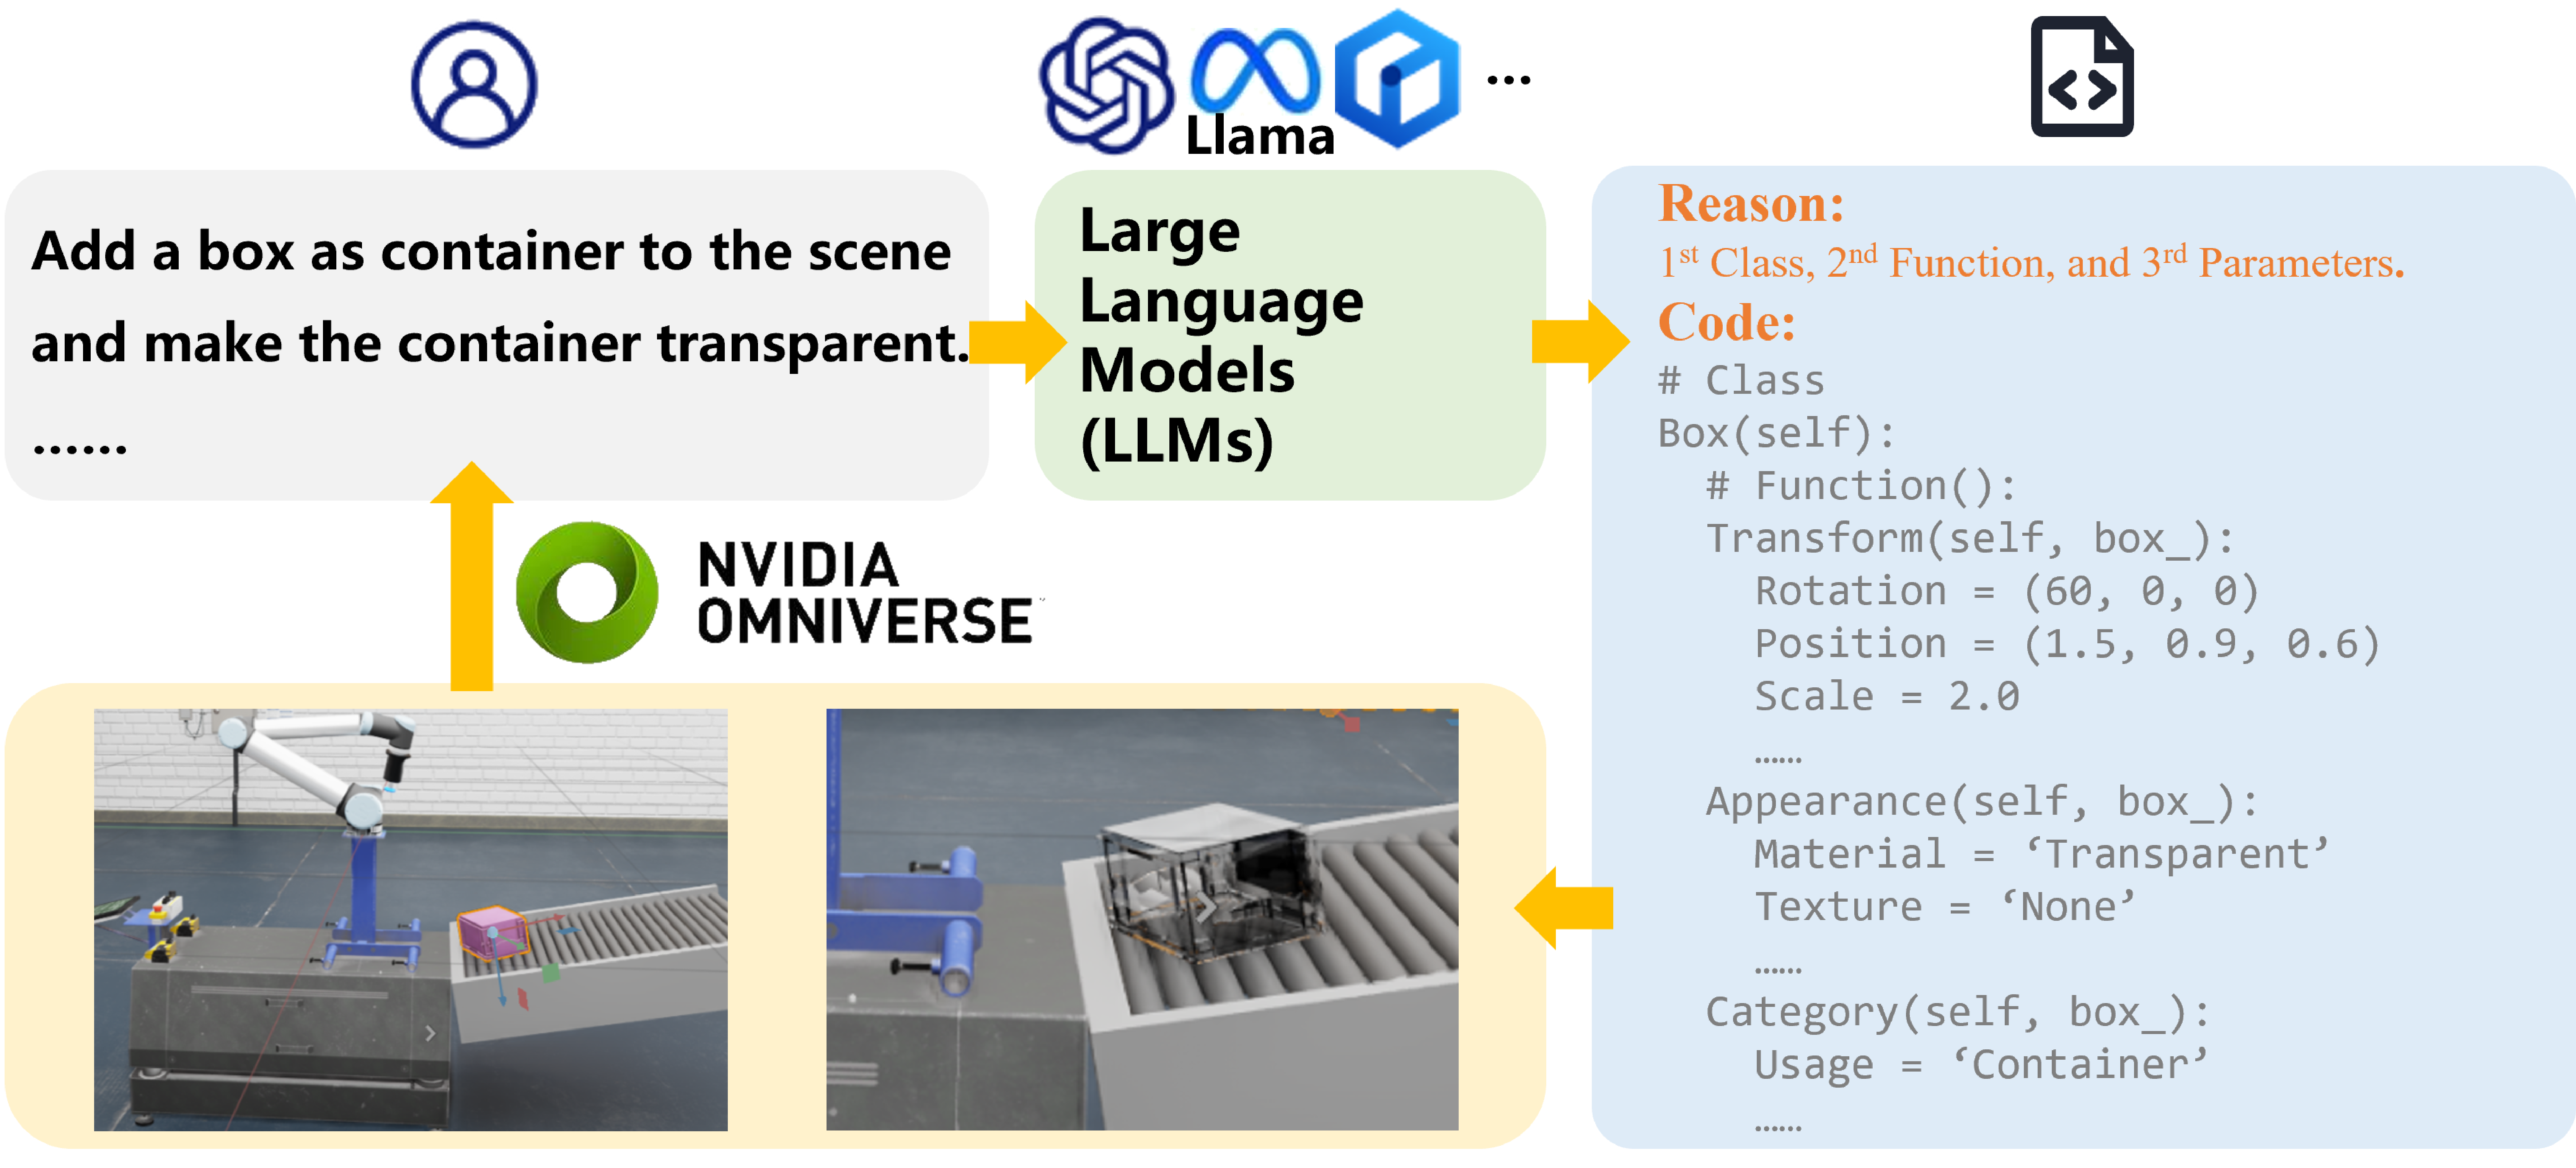
\includegraphics[width=0.88\textwidth]{5-Figures/nvidia_llm.pdf} 
    \caption{Digital twin code generation process for NVIDIA Omniverse using \glspl{LLM} \cite{Dong2024}.}
    \label{fig:llm_nvidia_omniverse}
\end{figure}

While \glspl{LLM} are flexible, their outputs can vary and sometimes contain errors. In industrial automation, deterministic behavior is essential for machine safety, meaning \gls{AI} tools are better suited as assistants for testing rather than for generating core machine structures.

\subsection{Synthesis of State-of-the-Art Approaches}

Comparing these methods highlights clear trade-offs. Model-driven methods \cite{Alexopoulos2025,Schaper2025} provide reliable structures, but usually end in pre-built scenes that cannot adapt dynamically at runtime. Data-driven methods \cite{Lugaresi2021,Garcia2023} are useful for legacy equipment, but lack detailed 3D geometry and kinematics. Generative \gls{AI} methods \cite{Dong2024} make initial scene drafting fast, but lack the consistency needed for control systems. Most importantly, nearly all existing solutions still require an engineer to manually assemble 3D assets in the simulation editor before compilation, making rapid reconfiguration on the factory floor difficult.

%=============================================================================
\section{Identified Research Gaps and Opportunities}
\label{sec:sota_gaps}
%=============================================================================

Reviewing the literature shows that while individual pieces of the \gls{DT} have progressed, integrating them into an automated procedural system remains an open challenge. Four main gaps stand out:

\begin{enumerate}
    \item \textbf{Gap 1: Fragmented Aspects vs. Unified Semantic Metamodel.}
    While 3D extraction tools \cite{Chowdhury2025,Dong2024} handle meshes without electrical \gls{IO} or control logic, semantic tools \cite{Gollner2022,Perez2025} manage properties without integrated 3D kinematics. An open submodel schema is needed that combines 3D meshes, kinematic limits, virtual \gls{IO} pins, and control logic rules in a single portable package.
    
    \item \textbf{Gap 2: Proprietary Formats vs. Standardized AAS Source of Truth.}
    Several automated systems generate custom scripts or prefabs tied to a specific simulation tool \cite{Alexopoulos2025,Schaper2025,Koch2024}. Keeping the standardized \gls{AAS} as the runtime source of truth ensures the digital asset remains interoperable across different factory systems.
    
    \item \textbf{Gap 3: Pre-Compiled Scenes vs. Runtime Procedural Instantiation.}
    In most game engine setups \cite{Alexopoulos2025,Pajpach2022,Garcia2025}, scenes must be manually compiled ahead of time, requiring software rebuilds whenever factory equipment changes. A runtime loader that ingests self-contained \gls{AASX} packages directly into memory eliminates this dependency.
    
    \item \textbf{Gap 4: Offline Simulation vs. Live Closed-Loop Synchronization.}
    Virtual commissioning tools \cite{Striffler2023,Schaper2025} support offline logic testing but lack online hardware synchronization, whereas \gls{IOT} dashboards stream telemetry without physics simulation. A unified framework should support both modes using the same asset description.
\end{enumerate}

To synthesize these gaps, \Cref{tab:sota_comparison} compares the proposed framework against leading approaches in the literature across key architectural capabilities.

\begin{table}[htbp]
    \centering
    \caption{Comparative analysis of state-of-the-art automated \gls{DT} frameworks.}
    \label{tab:sota_comparison}
    \renewcommand{\arraystretch}{1.2}
    \resizebox{\textwidth}{!}{%
    \begin{tabular}{lccccc}
        \toprule
        \textbf{Approach} & \textbf{Open Standard} & \textbf{Unified Schema} & \textbf{Procedural} & \textbf{Physics /} & \textbf{Live Hardware} \\
        & \textbf{(\gls{AAS} / \gls{AML})} & \textbf{(3D + \gls{IO} + Logic)} & \textbf{Runtime} & \textbf{Colliders} & \textbf{Synchronization} \\
        \midrule
        \textcite{Alexopoulos2025}   & \gls{AML}            & Partial (\gls{CAD} + \gls{AML})     & No (Pre-compiled) & Yes & No (Simulation only) \\
        \textcite{Schaper2025}       & \gls{AAS} / \gls{AML}      & No (\gls{FMU} focused)        & No (Offline \gls{VC})   & Yes & No (Offline \gls{SIL}) \\
        \textcite{Chowdhury2025}     & Proprietary    & No (Kinematics only)    & Partial (Editor)  & Yes & No (Offline) \\
        \textcite{Perez2025}         & \gls{AAS}            & No (Signals only)       & No                & No  & Yes (DataBridge) \\
        \textcite{Pajpach2023}       & \gls{AAS} / \gls{OPCUA}   & No (Separate models)    & No (Pre-compiled) & Yes & Yes (\gls{OPCUA} polling) \\
        \midrule
        \textbf{This Dissertation}   & \textbf{\gls{AAS} (\gls{IEC}~63278)} & \textbf{Yes (\gls{AASX} package)} & \textbf{Yes (100\% in-memory)} & \textbf{Yes} & \textbf{Yes (Dual-mode)} \\
        \bottomrule
    \end{tabular}%
    }
\end{table}

These gaps motivate the design and research goals of this dissertation. \Cref{cha:architecture} presents the conceptual architecture designed to address these challenges.